\documentclass[14pt,a4paper]{extarticle}
\usepackage{fontspec}
\usepackage{polyglossia}
\setmainlanguage{russian}
\setotherlanguage{english}

\setmainfont[Ligatures=TeX]{Times New Roman}
\setsansfont[Ligatures=TeX]{Arial}
\setmonofont{Consolas}

\newfontfamily\cyrillicfont[Ligatures=TeX]{Times New Roman}
\newfontfamily\cyrillicfontsf[Ligatures=TeX]{Arial}
\newfontfamily\cyrillicfonttt{Consolas}
\usepackage{setspace}
\onehalfspacing
\usepackage{geometry}
\geometry{left=30mm, right=15mm, top=20mm, bottom=20mm}
\usepackage{indentfirst}
\setlength{\parindent}{1.25cm}
\setlength{\parskip}{0pt}
%\usepackage{url}
\usepackage{xurl}
\urlstyle{same} % для переносов в ссылках
\usepackage{hyperref}
\usepackage{tabularx}
\usepackage{array}
\usepackage[table]{xcolor}
\definecolor{pastelgreen}{HTML}{B5EAD7}
\usepackage{booktabs}
\usepackage{ragged2e} % для justifying
\usepackage{graphicx}
\usepackage{float}
\usepackage{pdflscape}
\usepackage{fancyvrb}
\usepackage{amsmath}
\usepackage{amssymb}
\usepackage{wasysym}
\usepackage{caption}
\usepackage{enumitem}
\usepackage{fvextra}

\usepackage{listings}
\usepackage{xcolor}

\lstset{
    language=Python,
    numbers=left,
    numberstyle=\tiny,
    stepnumber=1,
    numbersep=5pt,
    frame=single,
    breaklines=true,
    backgroundcolor=\color{white},
    basicstyle=\ttfamily\small,
    keywordstyle=\color{blue},
    commentstyle=\color{gray},
    stringstyle=\color{orange},
    captionpos=b
}

\DefineVerbatimEnvironment{Code}{Verbatim}{
    fontsize=\small,
    breaklines=true,
    breakanywhere=true,
    frame=single,
    numbers=left,
    numbersep=6pt
}

\begin{document}
	
	\sloppy
	\thispagestyle{empty}
	\centering{
		МИНИСТЕРСТВО НАУКИ И ВЫСШЕГО ОБРАЗОВАНИЯ\\
		РОССИЙСКОЙ ФЕДЕРАЦИИ\\
		Федеральное государственное автономное образовательное учреждение высшего образования «Санкт-Петербургский политехнический университет Петра Великого»\\[10pt]
		Институт компьютерных наук и кибербезопасности\\
		Высшая школа технологий искусственного интеллекта\\
		02.03.01 Математика и компьютерные науки\\
		\vspace{\fill}
		{\large
			Отчёт по курсовой работе\\
			по дисциплине\\
			{\Large \bfseries Теоретические основы баз данных}\\
			{\Large <<Каталогизация экзопланет>>}\\
			\vspace{\fill}
		}
		
		
		{
			\flushright
			{\bfseries Выполнил:}\\
			студент группы 5130201/40003\\
			Джабраилов А.В.\\
			\hspace{9cm}Подпись: \hrulefill \\
			{\bfseries Принял:}\\
			К. тех. наук. доц., доц.\\
			Попов С.Г.\\
			\hspace{9cm}Подпись: \hrulefill \\
			
			\hspace{9cm}<<\rule{1.5cm}{0.4pt}>> \hrulefill\ 2026~г.
		}
		
		\centering{
			Санкт-Петербург, 2026
		}
	}
	
	%\flushleft
	\newpage
	%\justifying
	\justifying
    
	\section*{Реферат}
	\addcontentsline{toc}{section}{Реферат}
	Предметной областью данной работы является каталогизация экзопланет и связанных с ними астрономических объектов. Основная проблема заключается в разрозненности сведений об экзопланетах, звёздах, галактиках, телескопах и наблюдениях, что затрудняет централизованное хранение данных, сопоставление параметров объектов и выполнение аналитических запросов.

	В рамках работы спроектирована и реализована реляционная база данных, хранящая сведения о галактиках, звёздных скоплениях, звёздных и планетарных системах, звёздах, экзопланетах, телескопах, наблюдателях и событиях наблюдения. Для базы данных разработаны логическая и физическая схемы, выполнено заполнение тестовыми данными, а также сформированы SQL-запросы для получения аналитической информации по предметной области.

	Сформированы и выполнены девять запросов, включая выборку телескопов по параметрам наблюдаемых экзопланет, подсчёт наблюдавшихся звёзд, анализ распределений по классам звёзд и числу наблюдений, поиск стран с экстремальными значениями, сравнение активности наблюдателей, подсчёт наблюдений по странам и телескопам, а также обновление записей наблюдений. Для запросов приведены тексты SQL, реляционные формулы, последовательности выполнения, текстовые пояснения и фрагменты результатов.

	База данных содержит 273~166 записей в 9 таблицах. Для заполнения использовался язык Python с библиотекой \textit{psycopg2}; построение графиков результатов выполнено средствами языка R. Все запросы выполнялись в СУБД PostgreSQL на ноутбуке HP Pavilion Gaming Laptop 16-a0xxx с процессором Intel(R) Core(TM) i7-10750H CPU, 6 ядер, 2.60 ГГц, и 16 ГБ оперативной памяти.
	\newpage
	
	\tableofcontents
	
	\newpage
	
	\section*{Введение}
	\addcontentsline{toc}{section}{Введение}
	База данных (БД) --- совокупность структурированных данных, хранимых в соответствии со схемой и управляемых по единым правилам модели данных. Система управления базами данных (СУБД) --- программный комплекс, обеспечивающий создание БД, манипулирование данными (вставка, обновление, удаление, выборка), целостность, безопасность и надёжность хранения, а также средства администрирования.
	
	Разработка базы данных включает проектирование логической и физической структуры, реализацию схемы в выбранной СУБД и наполнение данными. Корректно спроектированная БД позволяет систематизировать большие объёмы информации, ускорить обработку запросов, снизить избыточность данных и обеспечить целостность при многопользовательском доступе.
	
	Данная работа посвящена проектированию и реализации реляционной базы данных для предметной области <<Каталогизация экзопланет>>. Предметная область охватывает хранение сведений об экзопланетах, звёздах, планетарных системах, звёздных системах, звёздных скоплениях, галактиках, телескопах, наблюдателях и событиях наблюдения. Такая база данных позволяет связывать астрономические объекты между собой, фиксировать параметры наблюдений и выполнять аналитические SQL-запросы по каталогизированным данным.
	
	В качестве СУБД используется PostgreSQL; заполнение базы данных реализовано на языке Python с использованием библиотеки psycopg2; выполнение запросов выполнено на языке SQL; построение графиков реализовано на языке R.
	
	\newpage
	
	\section{Постановка задачи}
	
	\textbf{Цель работы:} реализация функционирующей реляционной базы данных для предметной области <<Каталогизация экзопланет>> и выполнение заданных SQL-запросов.
	
	\textbf{Задачи работы:}
	\begin{enumerate}
		\item проанализировать предметную область каталогизации экзопланет;
		\item определить цели функционирования базы данных;
		\item выявить сущности, их атрибуты и связи;
		\item построить ER-диаграмму в нотации Чена;
		\item спроектировать схему базы данных и описать таблицы;
		\item перенести схему в СУБД PostgreSQL;
		\item реализовать программу заполнения базы данных тестовыми данными;
		\item сгенерировать базу данных объёмом не менее 250 тыс. записей;
		\item выполнить SQL-запросы к базе данных;
		\item сформировать реляционные формулы и последовательности выполнения запросов;
		\item построить графическое представление результатов запросов.
	\end{enumerate}
	
	\newpage
	
	\section{Аналитика}
	\subsection{Описание предметной области}
	\label{object-description}
	
	\textbf{Экзопланеты} --- это космические тела, идентифицируемые как планеты, находящиеся за пределами солнечной системы \cite{exoplanet}. Чтобы тело считалось планетой, оно должно удовлетворять трём критериям \cite{planet}: 
	\begin{itemize}
		\item оно должно вращаться вокруг звезды; 
		\item оно должно быть достаточно большим, чтобы силой гравитации поддерживать сферическую форму; 
		\item его гравитация не должна позволять другим объектам такого же размера приближаться к его орбите.
	\end{itemize}
	
	Однако некоторые космические тела, не вращающиеся вокруг какой-либо звезды, так же могут быть отнесены к планетам --- их называют планетами-изгоями \cite{exoplanet}.
	
	Большинство обнаруженных экзопланет расположены в относительно малой области нашей галактики, а именно в пределах тысяч световых лет от Солнечной системы. Например, ближайшая известная экзопланета, \textit{Proxima Centauri b}, находится на расстоянии 4 световых лет от нас. Планет в космосе больше, чем звёзд, однако задача их обнаружения гораздо сложнее, чем со звёздами, так как они не являются самосветящимися объектами, поэтому обнаружить экзопланету можно только косвенно, опираясь на звезду рядом с ней (например, заметив, что часть света звезды перекрывается каким-то телом или что звезда "покачивается" от гравитации другого тела, вращающегося вокруг него).
	
	Каталогизация экзопланет представляет собой многоэтапный процесс сбора, верификации и систематизации данных о них. С момента открытия первой подтверждённой экзопланеты в 1992 году их число превысило 6000 объектов \cite{exoplanet}, и с каждым годом темпы открытий ускоряются благодаря новым космическим миссиям и телескопам, в том числе тем, что расположены на орбите, а так же зондам. Однако рост объёма данных сопровождается фрагментацией информации: одни и те же планеты могут фигурировать в разных каталогах с разными параметрами, а сами параметры нередко противоречат друг другу из-за различий в методах наблюдений и обработки или разных дат последнего обновления информации.
	
	Основными участниками процесса каталогизации выступают астрономы-наблюдатели, астрофизики и кураторы каталогов. Наблюдатели регистрируют космические объекты с помощью телескопов, таких как космический телескоп «Кеплер», «Тесс» или наземные обсерватории вроде Ла-Силья в Чили \cite{lasilla}. Полученные данные передаются астрофизикам, которые интерпретируют их для расчёта физических параметров: массы, радиуса, орбитального периода и температуры поверхности. Завершающим этапом становится работа куратора каталога, который проверяет соответствие данных принятым стандартам, устраняет дубликаты и присваивает объекту уникальный идентификатор. В современных каталогах часть задач куратора выполняют автоматизированные системы, однако окончательная верификация по-прежнему требует участия человека.
	
	На сегодняшний день существует несколько независимых каталогов экзопланет, каждый со своей структурой хранения и правилами идентификации. Крупнейший из них --- \textit{NASA Exoplanet Archive} \cite{nasa-exoplanet-catalog} --- содержит данные о 6000 экзопланетах с изображениями. Альтернативный \textit{Open Exoplanet Catalogue} \cite{oec} содержит на 1000 экзопланет меньше, чем у NASA. Европейский архив \textit{Catalogue of Exoplanets} фокусируется на публикациях в рецензируемых журналах. Отсутствие единого формата приводит к тому, что одна и та же экзопланета может иметь разные характеристики в разных каталогах. Это обосновано тем, что при исследовании экзопланет сложно дать точную характеристику всем их параметрам: даже у первой открытой экзопланеты Kepler-186f не известны точные масса, состав и т.д. \cite{kepler}.
	
	Качество данных в каталоге определяется несколькими факторами. Во-первых, методом обнаружения: транзитный метод даёт точные значения радиуса, но не массы; метод радиальных скоростей, напротив, позволяет определить массу, но не размер. Во-вторых, количеством независимых подтверждений: планета, обнаруженная двумя разными телескопами, считается более надёжной. В-третьих, датой последнего измерения: параметры некоторых экзопланет уточняются спустя годы после открытия по мере накопления новых наблюдений.
	
	Существуют разные способы, активно используемые учёными для открытия экзопланет \cite{methods}. %Два основных метода --- это транзитный метод и метод радиальной скорости \cite{methods}.
	%Например, \textbf{метод транзитной скорости}: когда планета оказывается прямо между наблюдателем и звездой, вокруг которой она вращается, она частично заслоняет свет звезды. На короткое время свет звезды становится тусклее. Это незначительное изменение, но его достаточно, чтобы астрономы поняли, что вокруг далекой звезды вращается экзопланета. Этот метод называется транзитным. Например, так был обнаружен газовый гигант \textit{51 Pegasi b} \cite{methods}. Альтернативный метод --- \textbf{Метод радиальной скорости}: из-за гравитационного воздействия планет звезды раскачиваются в пространстве, что влияет на спектр света, который видят астрономы при наблюдении за звездой. На звезды влияет гравитационное притяжение планет, которые вращаются вокруг них, и при наблюдении в телескоп это влияет на спектр света звезды. Если звезда движется в направлении наблюдателя, ее спектр смещается в сторону синего. Если звезда удаляется от наблюдателя, ее спектр смещается в сторону красного. Третий метод --- \textbf{транзитная стереоскопия}: этот метод помогает изучать атмосферу экзопланет. После того как свет уловлен, его можно исследовать, чтобы определить состав атмосфер экзопланет. Это работает, как призма: если направить на нее белый свет, он разделится на радужный спектр. Ученые могут считывать цветовые полосы этого спектра, чтобы определить, какие молекулы в нем присутствуют. Так, например, у газового гиганта \textit{WASP-107b} обнаружили гелий в атмосфере --- это первый случай, когда этот элемент был найден в атмосфере экзопланет.
	
	\vspace{5pt}
	
	\begin{itemize}
		\item \textbf{Метод транзитной скорости}: когда планета оказывается прямо между наблюдателем и звездой, вокруг которой она вращается, она частично заслоняет свет звезды. На короткое время свет звезды становится тусклее. Это незначительное изменение, но его достаточно, чтобы астрономы поняли, что вокруг далекой звезды вращается экзопланета. Этот метод называется транзитным. Например, так был обнаружен газовый гигант \textit{51 Pegasi b}. \cite{methods}
		\item \textbf{Метод радиальной скорости}: из-за гравитационного воздействия планет звезды раскачиваются в пространстве, что влияет на спектр света, который видят астрономы при наблюдении за звездой. На звезды влияет гравитационное притяжение планет, которые вращаются вокруг них, и при наблюдении в телескоп это влияет на спектр света звезды. Если звезда движется в направлении наблюдателя, ее спектр смещается в сторону синего. Если звезда удаляется от наблюдателя, ее спектр смещается в сторону красного. Этот метод наблюдения называется методом измерения лучевой скорости.
		\item \textbf{Транзитная стереоскопия}: этот метод помогает изучать атмосферу экзопланет. После того как свет уловлен, его можно исследовать, чтобы определить состав атмосфер экзопланет. Это работает, как призма: если направить на нее белый свет, он разделится на радужный спектр. Ученые могут считывать цветовые полосы этого спектра, чтобы определить, какие молекулы в нем присутствуют. Так, например, у газового гиганта \textit{WASP-107b} обнаружили гелий в атмосфере --- это первый случай, когда этот элемент был найден в атмосфере экзопланет \cite{methods}.
	\end{itemize}
	
	Экзопланеты классифицируются по физическим характеристикам на несколько типов \cite{exoTypes}.%: \textbf{газовые гиганты} --- массивные планеты, обычно размером с Сатурн или Юпитер, но могут быть и больше. В этой категории планет есть подкатегории, например, горячие юпитеры --- газовые гиганты, вращающиеся вокруг звезды так быстро, что их температура достигает тысяч градусов Цельсия; \textbf{нептуновые планеты} размером с Нептун или Уран. Состав у них разнообразный, но все имеют атмосферу, преимущественно состояющую из водорода и гелия, а также имеют твёрдое ядро. Также существует подкатегория мини-Нептунов --- планет меньше Нептуна и больше Земли, но в Солнечной системе таких нет; \textbf{суперземли} --- каменистые планеты, массой больше Земли и меньше Нептуна; атмосфера у них может как быть, так и отсуствовать; \textbf{планеты земной группы} --- это планеты размером с Землю или меньше, состоящие из горных пород, силикатов (солей кремниевых кислот), воды или углерода. Дальнейшие исследования покажут, есть ли на некоторых из них атмосфера, океаны или другие признаки обитаемости.
	\label{types}
	\begin{itemize}
		\item \textbf{газовые гиганты} --- массивные планеты, обычно размером с Сатурн или Юпитер, но могут быть и больше. В этой категории планет есть подкатегории, например, горячие юпитеры --- газовые гиганты, вращающиеся вокруг звезды так быстро, что их температура достигает тысяч градусов Цельсия;
		\item \textbf{нептуновые планеты} размером с Нептун или Уран. Состав у них разнообразный, но все имеют атмосферу, преимущественно состояющую из водорода и гелия, а также имеют твёрдое ядро. Также существует подкатегория мини-Нептунов --- планет меньше Нептуна и больше Земли, но в Солнечной системе таких нет;
		\item \textbf{суперземли} --- каменистые планеты, массой больше Земли и меньше Нептуна; атмосфера у них может как быть, так и отсуствовать; 
		\item \textbf{планеты земной группы} --- это планеты размером с Землю или меньше, состоящие из горных пород, силикатов (солей кремниевых кислот), воды или углерода. Дальнейшие исследования покажут, есть ли на некоторых из них атмосфера, океаны или другие признаки обитаемости.
	\end{itemize}
	
	Создание унифицированной базы данных позволило бы решить ключевые проблемы современной каталогизации: устранить дублирование записей, обеспечить отслеживание истории изменений параметров и предоставить исследователям инструмент для поиска объектов по комбинации критериев — например, «все каменистые планеты в зоне обитаемости с массой от 0,8 до 1,5 массы Земли». Такая система особенно востребована в эпоху новых миссий, таких как космический телескоп «Джеймс Уэбб» \cite{webb}, запущенный в 2021 году, благодаря которым получится открыть множество других экзопланет и дать более точную оценку уже известным \cite{methods}.
	
	\subsection{Процессы}
	
	В данной предметной области имеются три процесса.
	
	\paragraph{1. Процесс каталогизации экзопланеты.} Астроном-наблюдатель обнаруживает космическое тело и передаёт информацию астрофизику, определяющему физические параметры этого тела. Данные передаются куратору каталога (архивариусу), который проверяет соответствие измерений стандартам и присваивает экзопланете идентификатор в соответствии с принятым в каталоге правилом.
	
	%Роли участников: наблюдатель, астрофизик, архивариус.
	
	\paragraph{2. Процесс обновления данных об экзопланете.} Обновление данных об экзопланете предполагает циклическое наблюдение её положения и состояния наблюдателем, вычисление текущих параметров и обнаружение различий с известными данными, после чего куратор каталога вносит скорректированные значения в каталог с указанием даты последнего измерения. Сегодня функцию архивариуса нередко выполняют автоматизированные системы.
	
	%Роли участников: наблюдатель, астрофизик, архивариус, автоматизированная система.
	
	\paragraph{3. Процесс извлечения данных об экзопланете.} Астроном, астрофизик, куратор каталога или астроном-любитель может извлечь данные об экзопланете из каталога, например, чтобы изучить её или сравнить данные с другими.
	
	%Роли участников: наблюдатель, астрофизик, архивариус, астроном-любитель.
	\subsection{Роли участников}
	В вышеперечисленных процессах присутствуют следующие участники:
	\begin{itemize}
		\item астроном-наблюдатель --- специалист, осуществляющий регистрацию космических объектов с помощью телескопов и регистрирующий первичные данные об их положении и движении;
		\item астрофизик --- учёный, интерпретирующий наблюдательные данные для определения физических параметров экзопланет: массы, радиуса, температуры и орбитальных характеристик;
		\item куратор каталога --- ответственный за верификацию поступающих данных, присвоение уникальных идентификаторов и соблюдение форматов хранения в соответствии со стандартами каталога;
		\item астроном-любитель --- непрофессиональный исследователь, использующий открытые данные для самостоятельного изучения экзопланет и потенциального участия в citizen science-проектах \cite{citizen-science-ru};
		%\item автоматизированная система \textit{???????????????????????)) ну типа она тоже вклад делает)))} --- программный комплекс, выполняющий предварительную обработку наблюдений, расчёт параметров и синхронизацию данных между распределёнными каталогами без участия человека.
	\end{itemize}
	
	\subsection{Цели функционирования базы данных}
	Цели функционирования базы данных следующие:
	\begin{itemize}
		%\item добавление и актуализация данных об экзопланетах и связанных с ними астрономических объектов и групп,
		%\item обеспечение долговременного хранения этих данных,
		%\item предоставление возможности поиска объектов по параметрам,
		%\item фиксация истории изменений измеренных параметров при повторных наблюдениях за экзопланетой.
		\item хранение данных о наблюдателях;
		\item хранение данных о первооткрывателях;
		\item хранение информации о наблюдении за экзопланетами;
		\item хранение использования телескопов наблюдателями;
		\item хранение принадлежности экзопланеты к более крупным космическим структурами.
	\end{itemize}
	
	\subsection{Сущности}
	В данной предметной области присутствуют сущности, перечисленные ниже.
	\begin{itemize}
		\item Экзопланета --- планета, находящаяся за пределами Солнечной системы. Термин и критерии, по которым определяется, является ли космическое тело планетой, даны в разделе \hyperref[object-description]{\underline{Описание предметной области}}.\\
		Они обладают следующими аттрибутами:
		\begin{itemize}
			\item уникальный идентификатор --- строка длиной до 100 символов, непустая, уникальная, состоящая из латинских букв, цифр, плюсов, минусов, дефисов, пробелов и точек, есть чувствительность к регистру (например, \textit{Kepler-186f}) \cite{names-standards};
			\item масса в массах Земли (M$ \oplus $) --- вещественное число, $> 0$, с точностью до 4 знаков после запятой;
			\item радиус в радиусах Земли (R$ \oplus $) --- вещественное число, $> 0$, с точностью до 4 знаков после запятой;
			\item орбитальный период в земных сутках (сут.) вещественное число, $> 0$, с точностью до 4 знаков после запятой;
			\item \hyperref[types]{\underline{тип}} планеты --- перечисление: \{Gas Giant, Neptunian, Superearth, Terrestial\};
			\item расстояние от нас в парсеках --- вещественное число, $\geq 0$, с точностью до 7 знаков после запятой;
			\item дата открытия --- дата в формате ГГГГ-ММ-ДД, 1992-01-01 -- текущая дата \cite{first-exoplanet-date}.
			\item дата последнего наблюдения --- календарная дата в формате ГГГГ-ММ-ДД, дата открытия -- текущая дата.
		\end{itemize}
		
		\item Звезда --- самосветящийся газовый шар, удерживаемый гравитацией, в котором происходят термоядерные реакции синтеза водорода в гелий.\\
		Обладает следующими атрибутами:
		\begin{itemize}
			\item уникальный идентификатор --- строка длиной до 100 символов, непустая, уникальная, состоящая из латинских букв, цифр, плюсов, минусов дефисов, пробелов и точек, есть чувствительность к регистру (например, \textit{Proxima Centauri});
			\item спектральный класс --- перечисление: $\{O, B, A, F, G, K, M, W, L, D\}$ \cite{stellar-classes}% × $\{0, 1 ,2 ,3, 4, 5, 6, 7, 8, 9\}$ × $\{I, II, III, IV, V\} $ \cite{stellar-classes};
			\item масса в массах Солнца (M$\odot$) --- вещественное число, $> 0$, с точностью до 3 знаков после запятой;
			\item радиус в радиусах Солнца (R$\odot$) --- вещественное число, $> 0$, с точностью до 3 знаков после запятой;
			\item температура поверхности в Кельвинах (К) --- целое число $> 0$;
			\item расстояние от нас в парсеках --- вещественное число, $\geq 0$, с точностью до 7 знаков после запятой.
		\end{itemize}
		
		\item Планетарная система --- совокупность планет и других небесных тел, гравитационно связанных и обращающихся вокруг одной звезды или звёздной системы.\\
		Обладает следующими атрибутами:
		\begin{itemize}
			\item уникальный идентификатор --- строка длиной до 100 символов, непустая, уникальная, состоящая из латинских букв, цифр, плюсов, минусов, дефисов, пробелов и точек, есть чувствительность к регистру (например, \textit{TRAPPIST-1});
			\item количество подтверждённых планет --- целое число, $\geq 1$;
			\item количество планет в зоне обитаемости --- целое число, $\geq 0$;
			\item расстояние от нас в парсеках --- вещественное число, $\geq 0$, с точностью до 7 знаков после запятой.
		\end{itemize}
		
		\item Звёздная система --- группа из одной или нескольких звёзд, связанных взаимным гравитационным притяжением и движущихся вокруг общего центра масс.\\
		Обладает следующими атрибутами:
		\begin{itemize}
			\item уникальный идентификатор --- строка длиной до 100 символов, непустая, уникальная, состоящая из латинских букв, цифр, плюсов, минусов, дефисов, пробелов и точек, есть чувствительность к регистру (например, \textit{TOI-1338});
			\item количество звёзд в звёздной системе --- целое число, $\geq 1$;
			\item количество подтверждённых планет --- целое число, $\geq 0$;
			\item количество планет в зоне обитаемости --- целое число, $\geq 0$;
			\item расстояние от нас в парсеках --- вещественное число, $\geq 0$, с точностью до 7 знаков после запятой.
		\end{itemize}
		
		\item Звёздное скопление --- группа звёзд, имеющих общее происхождение и удерживаемых вместе гравитацией.\\
		Обладает следующими атрибутами:
		\begin{itemize}
			\item уникальный идентификатор --- строка длиной до 100 символов, непустая, уникальная, состоящая из латинских букв, цифр, плюсов, минусов, дефисов, пробелов и точек, есть чувствительность к регистру (например, \textit{M4} \cite{M4});
			\item количество звёзд в звёздном скоплении --- целое число, $\geq 10$;
			\item количество подтверждённых планет --- целое число, $\geq 0$;
			\item расстояние от нас в парсеках --- вещественное число, $\geq 0$, с точностью до 7 знаков после запятой.
		\end{itemize}
		
		
		%\item Группа галактик (\textit{Galaxy Groups})--- небольшое скопление из нескольких десятков галактик, связанных гравитацией; пример --- Местная группа \cite{largeScale}.\\
		%Они обладают следующими аттрибутами:
		%\begin{itemize}
		%	\item уникальный идентификатор (например, \textit{Local Galaxy Group});
		%	\item количество галактик в группе;
		%	\item диаметр группы в мегапарсеках (МПс);
		%	\item доминирующая галактика (галактика с наибольшей массой);
		%	\item количество планет в зоне обитаемости.
		%\end{itemize}
		
		%\item Скопление галактик (\textit{Galaxy Clusters}) --- крупная структура из сотен или тысяч галактик, объединённых гравитацией и горячим межгалактическим газом \cite{largeScale}.\\
		%Они обладают следующими аттрибутами:
		%\begin{itemize}
		%	\item уникальный идентификатор (например, \textit{Veronica's Hair Cluster});
		%	\item количество галактик в скоплении;
		%	\item диаметр скопления в мегапарсеках (МПс);
		%	\item количество планет в зоне обитаемости.
		%\end{itemize}
		
		
		
		\item Галактика --- гигантская гравитационно связанная система из звёзд, газа, пыли и тёмной материи, имеющая характерную форму и структуру.\\
		Обладает следующими атрибутами:
		\begin{itemize}
			\item уникальный идентификатор --- строка длиной до 100 символов, непустая, уникальная, состоящая из латинских букв, цифр, плюсов, минусов, дефисов, пробелов и точек, есть чувствительность к регистру (например, \textit{The Milky Way});
			\item количество подтверждённых планет --- целое число, $\geq 0$;
			\item количество планет в зоне обитаемости --- целое число, $\geq 0$;
			\item расстояние от нас в парсеках --- вещественное число, $\geq 0$, с точностью до 7 знаков после запятой (для Млечного Пути = 0).
		\end{itemize}
		
		\item Телескоп --- инструмент, с помощью которого исследуют космос. В данном случае это телескоп, с помощью которого была обнаружена экзопланета, например, для \textit{WASP-107b} это \textit{Hubble}.\\
		Обладает следующими атрибутами:
		\begin{itemize}
			\item название телескопа --- строка длиной до 50 символов, непустая, уникальная, состоящая из латинских букв, цифр, дефисов, пробелов и точек, чувствительность к регистру (например, \textit{Hubble});
			\item тип --- перечисление: \{космический, наземный\};
			\item диаметр апертуры в метрах --- вещественное число, $> 0$, с точностью до 2 знаков после запятой;
			\item год ввода в эксплуатацию --- нижняя граница --- 1609 -- текущая дата;
			\item организация-оператор --- непустая строка длиной до 50 символов (например, \textit{NASA});
			\item количество планет, открытых телескопом --- целое число, $\geq 0$.
		\end{itemize}
		
		\item Наблюдатель --- астроном, наблюдающий за экзопланетами, или организация-оператор телескопа, которая наблюдает за экзопланетами, так как не все планеты наблюдаются вручную и только одним человеком.\\
		Обладает следующими атрибутами:
		\begin{itemize}
			\item уникальный идентификатор --- ФИО человека или название организации-оператора телескопа; строка длиной до 100 символов, непустая, уникальная, состоящая из латинских букв, цифр, дефисов, пробелов и точек, чувствительность к регистру (например, \textit\{NASA\});
			\item дата рождения / основания --- нижняя граница --- 1609 -- текущая дата;
			\item страна --- словарь, включающий в себя все страны;
			\item количество открытий --- целое число, $\geq 0$.
		\end{itemize}
	\end{itemize}

	%%%
	%\newpage
	%\special{papersize=420mm,297mm}
	%\geometry{left=30mm, right=15mm, top=20mm, bottom=20mm}

	\subsection{ER-диаграмма}
	Визуальное представление структуры базы данных, отображающее сущности, их атрибуты и связи между ними в виде ER-диаграммы представленно на рис. \ref{er}.
	%\begin{figure}[H]
	%	\centering
	%	
\includegraphics[width=0.85\linewidth]{er.drawio}
	%	\caption{ER-диаграмма}
	%	\label{er}
	%\end{figure}
	
	%\restoregeometry
	%\newpage
	%%%
	
	\clearpage
	\newgeometry{paperwidth=420mm,paperheight=297mm,margin=-2mm}
	
	\begin{landscape}
		\thispagestyle{empty}
		%\captionsetup{font=small,skip=4pt}
		
		\begin{figure}[!p]
			\centering
			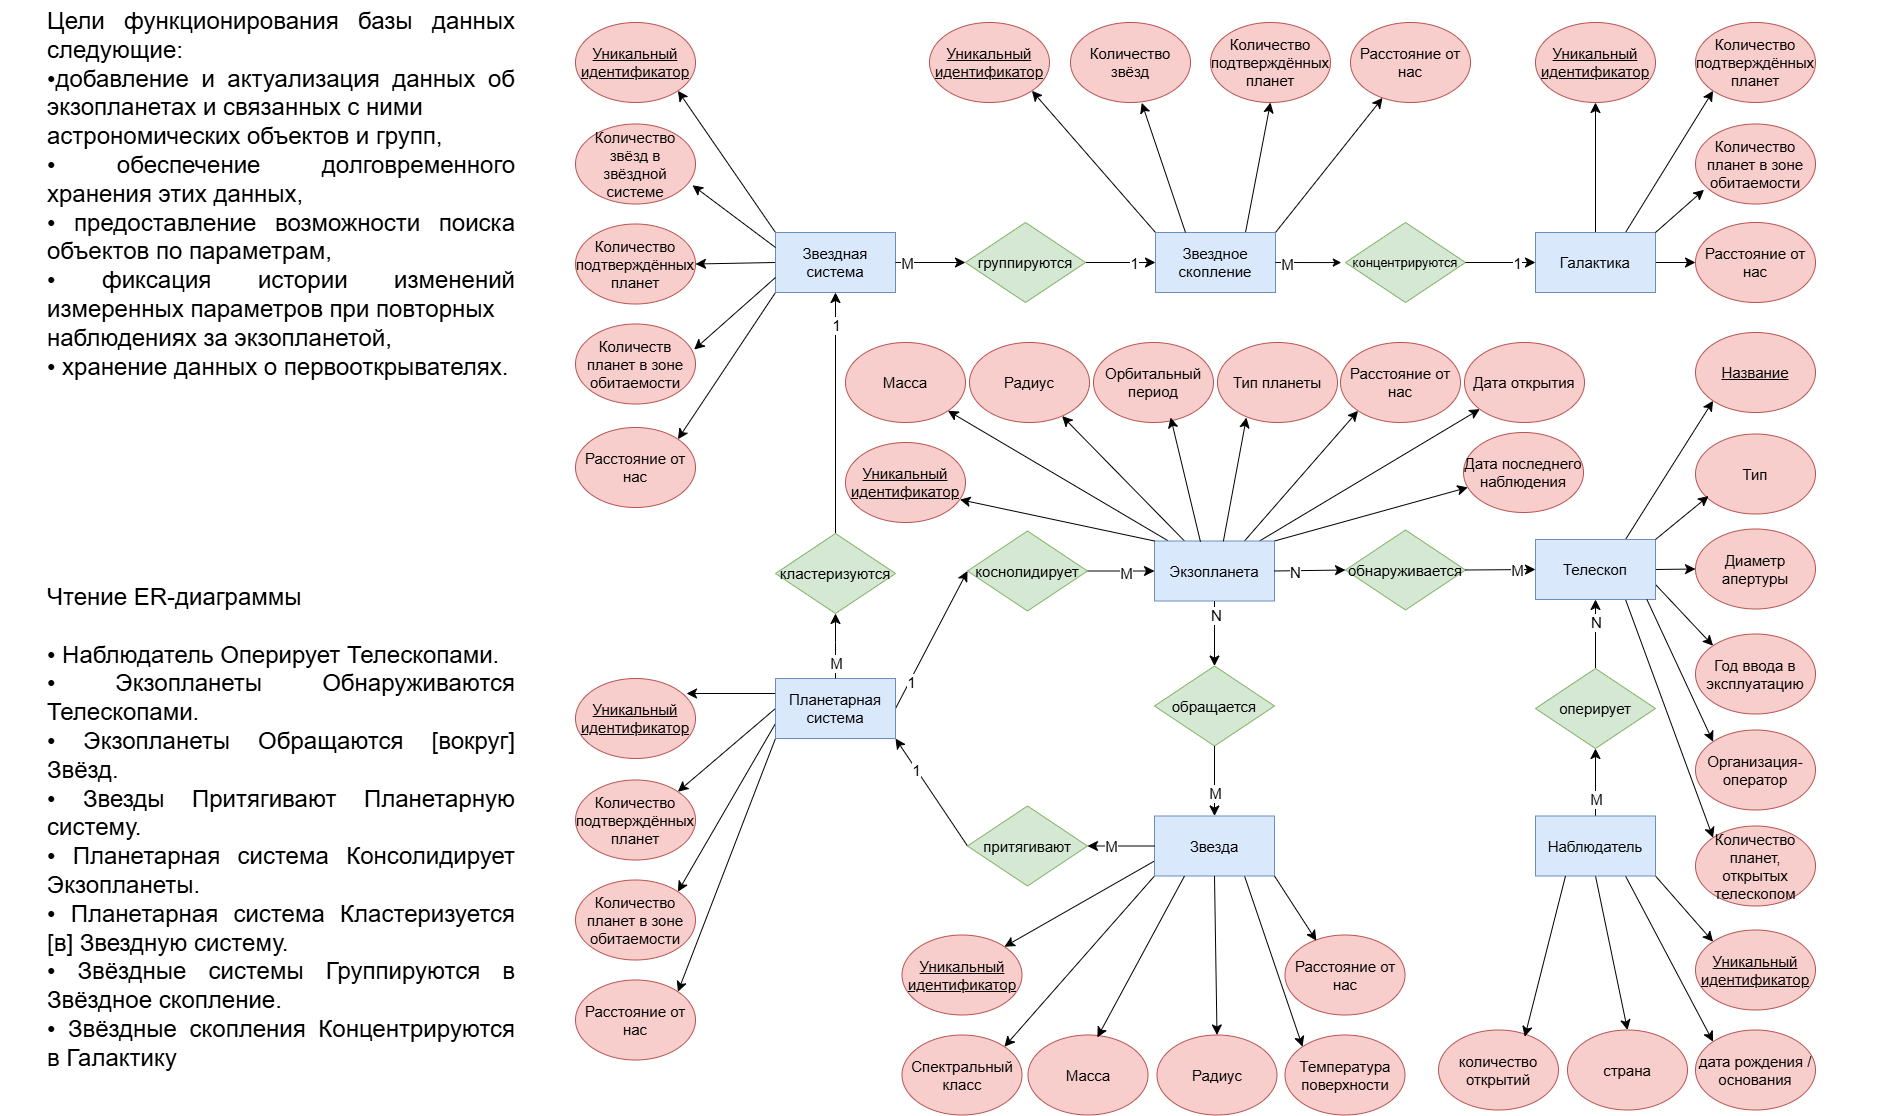
\includegraphics[width=\linewidth,height=\dimexpr\textheight-4\baselineskip\relax,keepaspectratio]{er.png}
			\caption{ER--диаграмма}
			\label{er}
		\end{figure}
	\end{landscape}
	
	\restoregeometry
	\clearpage
	
	
	\subsection{Чтение ER-диаграммы}
	\begin{itemize}
		\item Наблюдатель Оперирует Телескопами.
		\item Экзопланеты Обнаруживаются Телескопами.
		\item Экзопланеты Обращаются [вокруг] Звёзд.
		\item Звезды Притягивают Планетарную систему.
		\item Планетарная система Консолидирует Экзопланеты.
		\item Планетарная система Кластеризуется [в] Звездную систему.
		\item Звёздные системы Группируются в Звёздное скопление.
		\item Звёздные скопления Концентрируются в Галактику.
	\end{itemize}
	
	\subsection{Иерархия сущностей}
	Сущности рассматриваемой предметной области можно представить в виде следующей иерархической модели (рис. \ref{hy}):
	\begin{figure}[H]
		\centering
		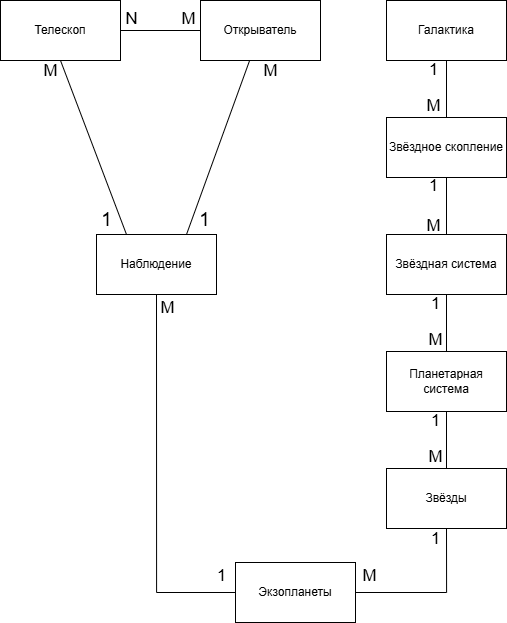
\includegraphics[width=0.85\linewidth]{hy}
		\caption{ER-диаграмма}
		\label{hy}
	\end{figure}
	
	\newpage

\section{Проектирование}

\subsection{Таблицы с описанием таблиц базы данных}

	В п. 1.4 были перечислены сущности, их атрибуты и домены.

	В следующих таблицах указаны метаданные полученной базы данных и обоснования доменов аттрибутов.

	\begin{table}[H]
    \centering
    \caption{Экзопланета}
    \small
    \begin{tabular}{|c|p{3.2cm}|p{2.6cm}|p{2.8cm}|p{1.5cm}|p{1.5cm}|c|}
\hline
№ & Название RU & Название EN & Тип атрибута & Тип ключа & Ссылка & Прим. \\
\hline
1 & экзопланета\_id & exo\_id & VARCHAR(30) & PK & - & NOT NULL \\
2 & масса & mass & DECIMAL(10,4) & - & - & NOT NULL \\
3 & радиус & radius & DECIMAL(10,4) & - & - & NOT NULL \\
4 & орбитальный\_ период & orb\_period & DECIMAL(10,4) & - & - & NOT NULL \\
5 & тип\_экзопланеты & exo\_type & ENUM & - & - & NOT NULL \\
6 & расстояние & dist & DECIMAL(12,6) & - & - & NOT NULL \\
7 & дата\_открытия & discov\_date & DATE & - & - & NOT NULL \\
8 & дата\_последнего\_ наблюдения & last\_obs\_date & DATE & - & - & NOT NULL \\
9 & система\_id & sys\_id & VARCHAR(30) & FK & Планета рная\_сис тема (system\_ id) & NOT NULL \\
\hline
\end{tabular}
\end{table}
	\begin{itemize}
		\item Идентификатор экзопланеты, звезды, планетарной системы, звёздной системы, звёздного
	скопления и галактики ограничен 30 символами, а названия космических объектов
	могут содержать буквенно-цифровые обозначения с дефисами и точками (например,
	\textit{Kepler-186f}, \textit{Proxima Centauri}). Это обосновано тем, что самое длинное
	название звезды --- \textit{SDSS J122906.70+112221.4} (24 символа), а названия экзопланет представляют собой название звезды + идентификатор экзопланеты,
	кот. может быть не более 5 символов, + 1 пробел, итого 30 символов.
		\item Масса, радиус и орбитальный период экзопланеты хранятся как \textit{DECIMAL(10,4)}.
		\item Расстояние от нас до экзопланеты хранится в парсеках как \textit{DECIMAL(12,6)} для обеспечения точности до
	6 знаков после запятой, так как расстояния в световых годах указываются с точностью не более 2 знаков после запятой (до ближайшего объекта, расстояние до которого известно с наибольшей точностью, --- Proxima Centauri b --- расстояние составляет 4,24 светового года), парсек в световых годах указан с точностью до 4 знаков после запятой, а результат их умножения будет содержать максимум 6 знаков после запятой.
		\item Дата открытия и дата последнего наблюдения хранятся как \textit{DATE} в формате
	ГГГГ-ММ-ДД. Минимальная дата обоснована датой открытия первой экзопланеты (1992-01-01). Максимальная дата обоснована тем, что объект, не открытый сейчас, не является открытым в принципе, потому эта дата не может превышать сегодняшнюю дату.
		\item Типы экзопланет хранятся как \textit{ENUM} с фиксированным набором
	значений: \{Gas Giant, Neptunian, Superearth, Terrestial\}.
	\end{itemize}

	\begin{table}[H]
    \centering
    \caption{Звезда}
    \small
    \begin{tabular}{|c|p{3.2cm}|p{2.6cm}|p{2.8cm}|p{1.5cm}|p{1.5cm}|c|}
\hline
№ & Название RU & Название EN & Тип атрибута & Тип ключа & Ссылка & Прим. \\
\hline
1 & звезда\_id & star\_id & VARCHAR(30) & PK & - & NOT NULL \\
2 & класс & class & ENUM & - & - & NOT NULL \\
3 & масса & mass & DECIMAL(5,2) & - & - & NOT NULL \\
4 & радиус & radius & DECIMAL(10,4) & - & - & NOT NULL \\
5 & температура & temp & INT & - & - & NOT NULL \\
6 & расстояние & dist & DECIMAL(16,6) & - & - & NOT NULL \\
7 & система\_id & sys\_id & VARCHAR(30) & FK & Планета рная\_ система (system\_ id) & NOT NULL \\
\hline
\end{tabular}
\end{table}

	\begin{itemize}
		\item Масса звезды хранится как \textit{DECIMAL(5,2)}, т.к. самая массивная звезда \textit{R136a1} имеет массу 150--200 масс Солнца (т.е. 3 целых числа), а двух знаков после запятой достаточно для точности размеров ближайших звезд.
		\item Расстояние до звезды хранится как \textit{DECIMAL(16,6)} --- 10 целых знаков (самая далекая звезда находится на расстоянии 8.6 млрд парсек), 6 знаков после запятой для точности (так же, как с экзопланетами).
		\item Температура поверхности звезды хранится как целое число (\textit{INT}), так как в
	астрономических каталогах температура указывается без дробной части.
		\item Спектральный класс звезды хранится как \textit{VARCHAR(5)} для представления
	комбинированного класса (самый длинный класс может состоять из пяти символов, например, \textit{M5III}).
	\end{itemize}

	\begin{table}[H]
    \centering
    \caption{Планетарная система}
    \small
\begin{tabular}{|c|p{3.2cm}|p{2.6cm}|p{2.8cm}|p{1.5cm}|p{1.5cm}|c|}
\hline
№ & Название RU & Название EN & Тип атрибута & Тип ключа & Ссылка & Прим. \\
\hline
1 & система\_id & system\_id & VARCHAR(30) & PK & - & NOT NULL \\
2 & подтверждённых\_ планет & conf\_plan & INT & - & - & NOT NULL \\
3 & планет\_в\_зоне\_ обитаемости & hab\_plan & INT & - & - & NOT NULL \\
4 & расстояние & distance & DECIMAL(12,6) & - & - & NOT NULL \\
5 & звёздная\_система\_ id & stell\_sys\_id & VARCHAR(30) & FK & Звёздная \_система (stellar\_ id) & NOT NULL \\
\hline
\end{tabular}
\end{table}

	\begin{itemize}
		\item Количество подтверждённых планет, планет в зоне обитаемости хранится как целое число (\textit{INT}) и имеют минимальные значения, соответствюущие данным астрономическим объектам.
	\end{itemize}

	\begin{table}[H]
    \centering
    \caption{Звёздная система}
    \small
\begin{tabular}{|c|p{3.2cm}|p{2.6cm}|p{2.8cm}|p{1.5cm}|p{1.5cm}|c|}
\hline
№ & Название RU & Название EN & Тип атрибута & Тип ключа & Ссылка & Прим. \\
\hline
1 & звёздная\_система\_ id & stellar\_id & VARCHAR(30) & PK & - & NOT NULL \\
2 & количество\_звёзд & stars\_count & INT & - & - & NOT NULL \\
3 & подтверждённых\_ планет & conf\_plan & INT & - & - & NOT NULL \\
4 & планет\_в\_зоне\_ обитаемости & hab\_plan & INT & - & - & NOT NULL \\
5 & расстояние & dist & DECIMAL(12,6) & - & - & NOT NULL \\
6 & кластер\_id & cluster\_id & VARCHAR(30) & FK & Кластер (cluster\_ id) & NOT NULL \\
\hline
\end{tabular}
\end{table}

	\begin{itemize}
		\item Количество подтверждённых планет, планет в зоне обитаемости, звёзд хранится как целое число (\textit{INT}) и имеют минимальные значения, соответствюущие данным астрономическим объектам.
	\end{itemize}

	\begin{table}[H]
    \centering
    \caption{Кластер}
    \small
\begin{tabular}{|c|p{3.2cm}|p{2.6cm}|p{2.8cm}|p{1.5cm}|p{1.5cm}|c|}
\hline
№ & Название RU & Название EN & Тип атрибута & Тип ключа & Ссылка & Прим. \\
\hline
1 & кластер\_id & cluster\_id & VARCHAR(30) & PK & - & NOT NULL \\
2 & количество\_звёзд & stars\_count & INT & - & - & NOT NULL \\
3 & подтверждённых\_ планет & conf\_plan & INT & - & - & NOT NULL \\
4 & планет\_в\_зоне\_ обитаемости & hab\_plan & INT & - & - & NOT NULL \\
5 & расстояние & dist & DECIMAL(12,6) & - & - & NOT NULL \\
6 & галактика\_id & galaxy\_id & VARCHAR(30) & FK & Галакти ка (galaxy\_ id) & NOT NULL \\
\hline
\end{tabular}
\end{table}

	\begin{itemize}
		\item Количество подтверждённых планет, звёзд хранится как целое число (\textit{INT}) и имеют минимальные значения, соответствюущие данным астрономическим объектам (например, звёздное скопление содержит как минимум 10 звёзд по определению, поэтому это число является минимальным значением данного поля для звёздных скоплений).
	\end{itemize}

	\begin{table}[H]
    \centering
    \caption{Галактика}
    \small
\begin{tabular}{|c|p{3.2cm}|p{2.6cm}|p{2.8cm}|p{1.5cm}|p{1.5cm}|c|}
\hline
№ & Название RU & Название EN & Тип атрибута & Тип ключа & Ссылка & Прим. \\
\hline
1 & галактика\_id & galaxy\_id & VARCHAR(30) & PK & - & NOT NULL \\
2 & подтверждённых\_ планет & conf\_plan & INT & - & - & NOT NULL \\
3 & планет\_в\_зоне\_ обитаемости & hab\_plan & INT & - & - & NOT NULL \\
4 & расстояние & dist & DECIMAL(12,6) & - & - & NOT NULL \\
\hline
\end{tabular}
\end{table}

	\begin{itemize}
		\item Количество подтверждённых планет и планет в зоне обитаемости хранится как целое число (\textit{INT}) и имеют минимальные значения, соответствюущие данным астрономическим объектам.
	\end{itemize}

	\begin{table}[H]
    \centering
    \caption{Телескоп}
    \small
\begin{tabular}{|c|p{3.2cm}|p{2.6cm}|p{2.8cm}|p{1.5cm}|p{1.5cm}|c|}
\hline
№ & Название RU & Название EN & Тип атрибута & Тип ключа & Ссылка & Прим. \\
\hline
1 & телескоп\_id & tele\_id & VARCHAR(47) & PK & - & NOT NULL \\
2 & тип\_телескопа & tele\_type & ENUM & - & - & NOT NULL \\
3 & апертура & aper & DECIMAL(6,2) & - & - & NOT NULL \\
4 & дата\_создания & com\_year & INT & - & - & NOT NULL \\
5 & оператор & oper & VARCHAR(81) & - & - & NOT NULL \\
6 & открыто\_планет & discov\_plan & INT & - & - & NOT NULL \\
\hline
\end{tabular}
\end{table}

	\begin{itemize}
		\item Название телескопа ограничено 47 символами. Самое длинное название телескопа: \textit{Atacama Large Millimeter/submillimeter Array}.
		\item Диаметр апертуры телескопа хранится как \textit{DECIMAL(6,2)} с точностью до
	2 знаков после запятой.
		\item Год ввода в эксплуатацию хранится как целое число (\textit{INT}) в диапазоне от 1609 до
	текущего года.
		\item Организация-оператор телескопа ограничена 81 символами. Самое длинное название организации-оператора
		телескопа: \textit{European Southern Observatory for Astronomical Research in the Southern Hemisphere}.
		\item Типы телескопов хранятся как \textit{ENUM}, их значения: \{космический, наземный\}.
	\end{itemize}

	\begin{table}[H]
    \centering
    \caption{Наблюдатель}
    \small
\begin{tabular}{|c|p{3.2cm}|p{2.6cm}|p{2.8cm}|c|p{1.5cm}|c|}
\hline
№ & Название RU & Название EN & Тип атрибута & Тип ключа & Ссылка & Прим. \\
\hline
1 & наблюдатель\_id & observer\_id & VARCHAR(100) & PK & - & NOT NULL \\
2 & дата\_рождения & bday & DATE & - & - & NOT NULL \\
3 & страна & country & ENUM & - & - & NOT NULL \\
4 & открытий & discovs & INT & - & - & NOT NULL \\
\hline
\end{tabular}
\end{table}

	\begin{itemize}
		\item Название наблюдателя (ФИО или организация) ограничено 100 символами.
		\item Страна наблюдателя ограничена 56 символами. Самое длинное название страны:
		\textit{The United Kingdom of Great Britain and Northern Ireland}.
	\end{itemize}

	\begin{table}[H]
    \centering
    \caption{Наблюдение}
    \small
\begin{tabular}{|c|p{3.2cm}|p{2.6cm}|p{2.8cm}|p{1.5cm}|p{1.5cm}|c|}
\hline
№ & Название RU & Название EN & Тип атрибута & Тип ключа & Ссылка & Прим. \\
\hline
1 & наблюдение\_id & observation\_id & VARCHAR(30) & PK & - & NOT NULL \\
2 & экзопланета\_id & exo\_id & VARCHAR(30) & FK & Экзоп- ланета (exo\_id) & NOT NULL \\
3 & телескоп\_id & tele\_id & VARCHAR(47) & FK & Телескоп (tele\_id) & NOT NULL \\
4 & наблюдатель\_id & observer\_id & VARCHAR(100) & FK & Наблюда- тель (observer \_id) & NOT NULL \\
5 & дата\_наблюдения & obs\_date & DATE & - & - & NOT NULL \\
\hline
\end{tabular}
\end{table}

	\begin{itemize}
		\item Идентификатор наблюдения хранится как \textit{VARCHAR(30)} и представляет собой искусственный ключ. В отличие от других сущностей, наблюдение является событием, которое не имеет устойчивого естественного идентификатора, поэтому использование составного ключа (экзопланета, телескоп, наблюдатель, дата) является избыточным и усложняет структуру базы данных. Ограничение в 30 символов выбрано для унификации с другими идентификаторами.
	\end{itemize}

	\newpage

\subsection{Лингвистическое описание схемы базы данных}

\begin{enumerate}
    \item Галактика (галактика\_id(VARCHAR(30)), подтверждённых\_планет(INT), планет\_в\_зоне\_обитаемости(INT), расстояние(DECIMAL(12, 6))).

    \item Кластер (кластер\_id(VARCHAR(30)), количество\_звёзд(INT), подтверждённых\_планет(INT), планет\_в\_зоне\_обитаемости(INT), расстояние(DECIMAL(12, 6)), галактика\_id(VARCHAR(30))).

    \item Звёздная система (звёздная\_система\_id(VARCHAR(30)), количество\_звёзд(INT), подтверждённых\_планет(INT), планет\_в\_зоне\_обитаемости(INT), расстояние(DECIMAL(12, 6)), кластер\_id(VARCHAR(30))).

    \item Планетарная система (система\_id(VARCHAR(30)), подтверждённых\_планет(INT), планет\_в\_зоне\_обитаемости(INT), расстояние(DECIMAL(12, 6)), звёздная\_система\_id(VARCHAR(30))).

    \item Класс звезды (класс\_id(SERIAL), класс(VARCHAR(5))).

    \item Звезда (звезда\_id(VARCHAR(30)), класс\_id(INT), масса(DECIMAL(5, 2)), радиус(DECIMAL(10, 4)), температура(INT), расстояние(DECIMAL(16, 6)), система\_id(VARCHAR(30))).

    \item Тип экзопланеты (тип\_экзопланеты\_id(SERIAL), тип\_экзопланеты(VARCHAR(30))).

    \item Экзопланета (экзопланета\_id(VARCHAR(30)), масса(DECIMAL(10, 4)), радиус(DECIMAL(10, 4)), орбитальный\_период(DECIMAL(10, 4)), тип\_экзопланеты\_id(INT), расстояние(DECIMAL(12, 6)), дата\_открытия(DATE), дата\_последнего\_наблюдения(DATE), система\_id(VARCHAR(30))).

    \item Тип телескопа (тип\_телескопа\_id(SERIAL), тип\_телескопа(VARCHAR(30))).

    \item Телескоп (телескоп\_id(VARCHAR(47)), тип\_телескопа\_id(INT), апертура(DECIMAL(6, 2)), дата\_создания(INT), оператор(VARCHAR(81)), открыто\_планет(INT)).

    \item Страна (страна\_id(SERIAL), страна(VARCHAR(60))).

    \item Наблюдатель (наблюдатель\_id(VARCHAR(100)), дата\_рождения(DATE), страна\_id(INT), открытий(INT)).

    \item Наблюдение (наблюдение\_id(VARCHAR(30)), экзопланета\_id(VARCHAR(30)), телескоп\_id(VARCHAR(47)), наблюдатель\_id(VARCHAR(100)), дата\_наблюдения(DATE)).
\end{enumerate}

\subsection{Диаграммы базы данных}

	На рис. \ref{ru} изображена схема базы данных на русском языке.

	На рис. \ref{en} изображена схема базы данных на русском языке.

	На рис. \ref{order} изображён порядок заполнения таблиц базы данных.

\clearpage

	\newgeometry{paperwidth=420mm,paperheight=297mm,margin=-2mm}
	
	\begin{landscape}
		\thispagestyle{empty}
		%\captionsetup{font=small,skip=4pt}
		
		\begin{figure}[!p]
			\centering
			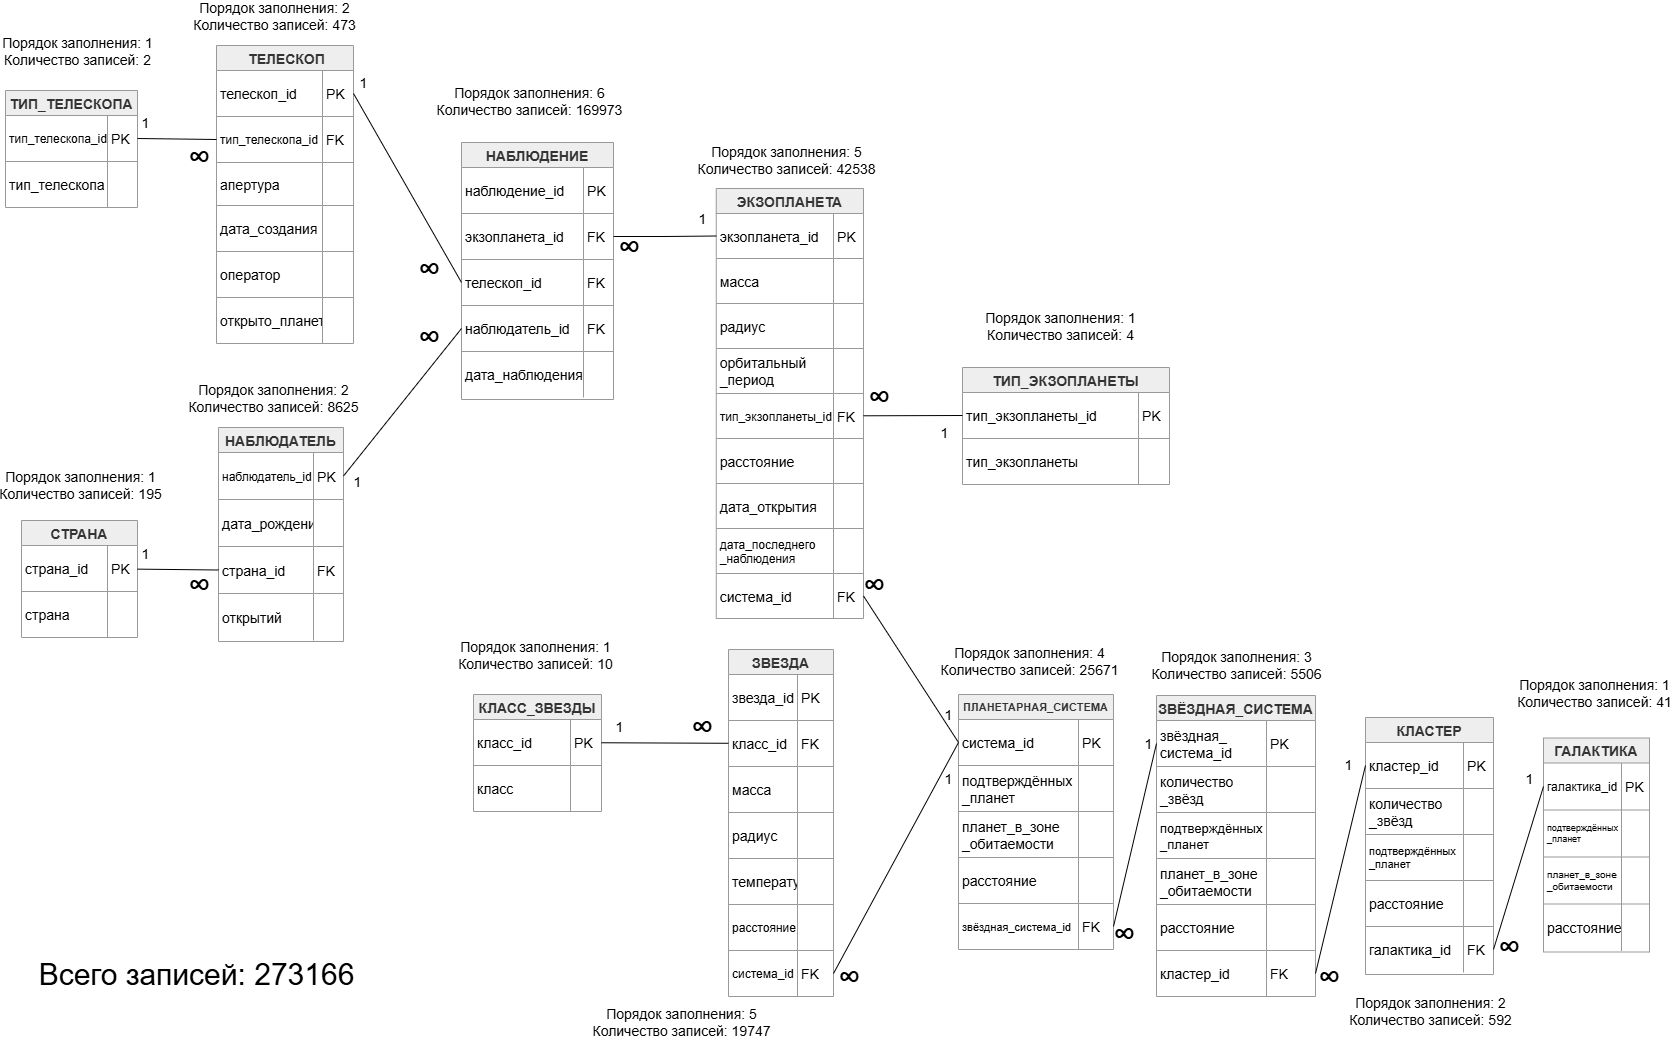
\includegraphics[width=0.9\linewidth,height=\dimexpr\textheight-4\baselineskip\relax,keepaspectratio]{ru.png}
			\caption{Диаграмма таблиц на русском языке.}
			\label{ru}
		\end{figure}
	\end{landscape}
	
	\restoregeometry
	\clearpage

\clearpage

	\newgeometry{paperwidth=420mm,paperheight=297mm,margin=-2mm}
	
	\begin{landscape}
		\thispagestyle{empty}
		%\captionsetup{font=small,skip=4pt}
		
		\begin{figure}[!p]
			\centering
			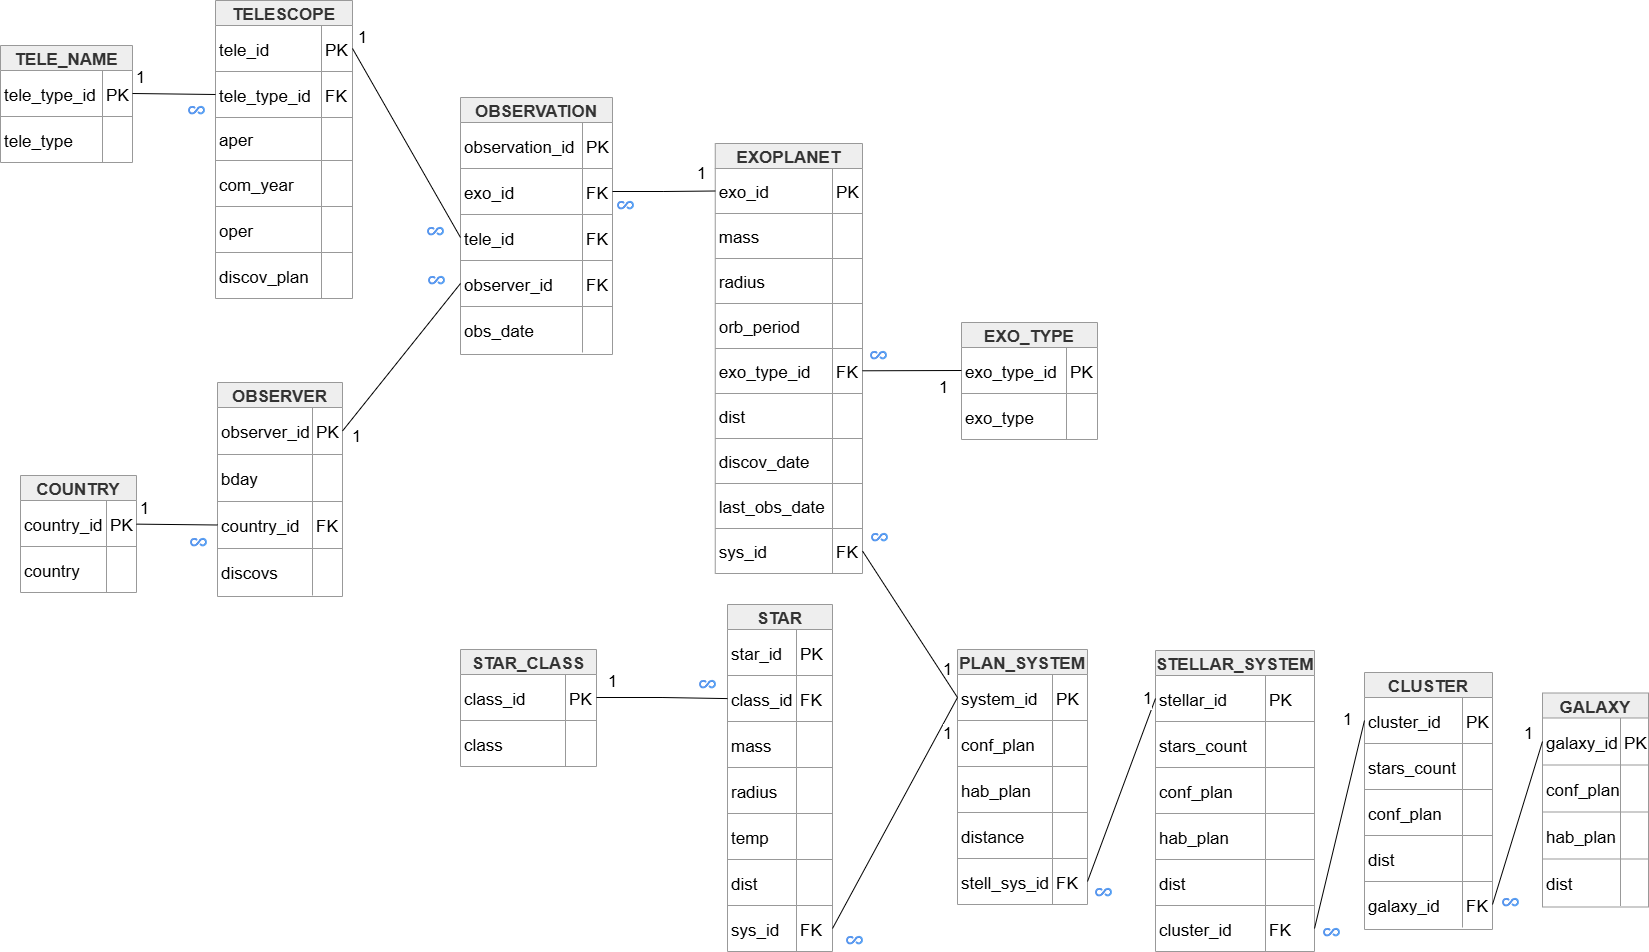
\includegraphics[width=0.9\linewidth,height=\dimexpr\textheight-4\baselineskip\relax,keepaspectratio]{en.png}
			\caption{Диаграмма таблиц на английском языке.}
			\label{en}
		\end{figure}
	\end{landscape}
	
	\restoregeometry
	
\clearpage

\clearpage
	\newgeometry{paperwidth=420mm,paperheight=297mm,margin=-2mm}
	
	\begin{landscape}
		\thispagestyle{empty}
		%\captionsetup{font=small,skip=4pt}
		
		\begin{figure}[!p]
			\centering
			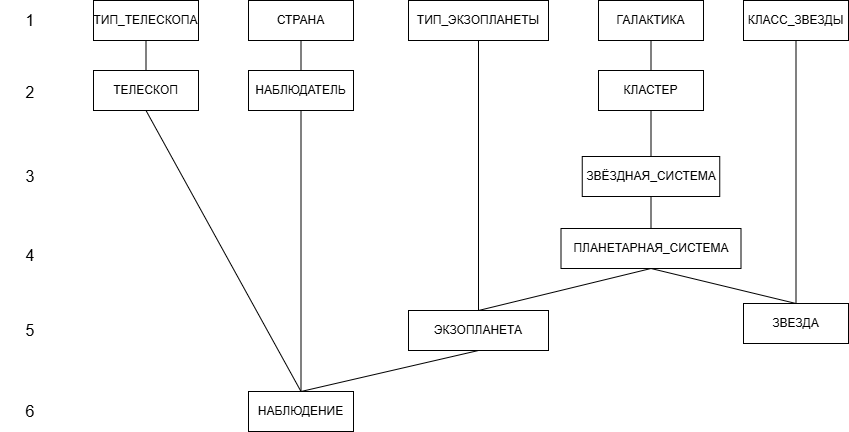
\includegraphics[width=0.9\linewidth,height=\dimexpr\textheight-4\baselineskip\relax,keepaspectratio]{order.png}
			\caption{Диаграмма порядка заполнения таблиц.}
			\label{order}
		\end{figure}
	\end{landscape}
	
	\restoregeometry
\clearpage

\newpage

\section{Программирование}

\subsection{Генерация тестовых данных}

Для заполнения базы данных использовался язык программирования Python и библиотека \textit{psycopg2}, предназначенная для подключения к PostgreSQL и выполнения SQL-запросов из Python-программы. Для генерации фиктивных данных применялась стандартная библиотека \textit{random}, а для работы с календарными датами использовались классы \textit{date} и \textit{timedelta} из модуля \textit{datetime}.

Программа выполняет подключение к базе данных, очищает существующие таблицы, генерирует случайное количество записей в диапазоне от 200~000 до 300~000, после чего последовательно заполняет таблицы в порядке, соответствующем иерархии внешних ключей.

\begin{lstlisting}[caption={Подключение к базе данных}]
import psycopg2
from datetime import date, timedelta
import random

conn = psycopg2.connect(dbname="mydb", user="postgres")
cur = conn.cursor()
\end{lstlisting}

Перед генерацией новых данных выполняется очистка таблиц с помощью оператора \textit{TRUNCATE}. Таблицы перечислены в порядке от наиболее зависимых к родительским, а параметр \textit{CASCADE} позволяет завершать \textit{TRUNCATE} без ошибок, убирая связи между таблицами, чтобы не возникали ошибки.

\begin{lstlisting}[caption={Очистка таблиц перед генерацией}]
cur.execute("""
    TRUNCATE TABLE
        observation,
        exoplanet,
        star,
        telescope,
        observer,
        plan_system,
        stellar_system,
        cluster,
        galaxy
    CASCADE;
""")
\end{lstlisting}

Для генерации значений используются вспомогательные функции. Функция \textit{random\_date} создаёт случайную дату в заданном диапазоне. Функция \textit{random\_decimal} возвращает случайное вещественное число без дополнительного округления в Python. Функция \textit{make\_id} формирует строковые идентификаторы объектов по заданному префиксу и номеру.

\begin{lstlisting}[caption={Вспомогательные функции генерации}]
def random_date(start_date, end_date):
    days = (end_date - start_date).days
    return start_date + timedelta(days=random.randint(0, days))


def random_decimal(min_value, max_value):
    return random.uniform(min_value, max_value)


def make_id(prefix, number, width=5):
    return f"{prefix}_{number:0{width}d}"
\end{lstlisting}

Количество записей в основных таблицах выбирается случайно. При этом программа контролирует итоговый объём данных: сумма записей должна находиться в диапазоне от 200~000 до 300~000 (задано константами). Количество наблюдений оценивается приблизительно как произведение количества экзопланет на среднее число наблюдений для одной экзопланеты.

\begin{lstlisting}[caption={Генерация случайного количества записей}]
TARGET_MIN = 200_000
TARGET_MAX = 300_000

while True:
    GALAXIES_COUNT = random.randint(30, 70)
    CLUSTERS_COUNT = random.randint(300, 700)
    STELLAR_SYSTEMS_COUNT = random.randint(3000, 7000)
    PLAN_SYSTEMS_COUNT = random.randint(15000, 30000)
    STARS_COUNT = random.randint(15000, 30000)
    EXOPLANETS_COUNT = random.randint(30000, 50000)
    TELESCOPES_COUNT = random.randint(200, 500)
    OBSERVERS_COUNT = random.randint(7000, 15000)

    estimated_observations = EXOPLANETS_COUNT * 4

    estimated_total = (
        GALAXIES_COUNT
        + CLUSTERS_COUNT
        + STELLAR_SYSTEMS_COUNT
        + PLAN_SYSTEMS_COUNT
        + STARS_COUNT
        + EXOPLANETS_COUNT
        + TELESCOPES_COUNT
        + OBSERVERS_COUNT
        + estimated_observations
    )

    if TARGET_MIN <= estimated_total <= TARGET_MAX:
        break
\end{lstlisting}

После выбора количества записей дополнительно проверяется выполнение ограничений предметной области. В каждом звёздном скоплении должно быть не менее десяти звёзд, не менее одной планетарной системы и не менее одной звёздной системы. Если случайно выбранные значения не удовлетворяют этим условиям, они автоматически увеличиваются до минимально допустимых.

\begin{lstlisting}[caption={Проверка минимальных требований к иерархии}]
if STARS_COUNT < CLUSTERS_COUNT * 10:
    STARS_COUNT = CLUSTERS_COUNT * 10

if PLAN_SYSTEMS_COUNT < CLUSTERS_COUNT:
    PLAN_SYSTEMS_COUNT = CLUSTERS_COUNT

if STELLAR_SYSTEMS_COUNT < CLUSTERS_COUNT:
    STELLAR_SYSTEMS_COUNT = CLUSTERS_COUNT
\end{lstlisting}

Заполнение базы данных выполняется в шесть уровней. Сначала задаются справочные значения: типы телескопов, страны, типы экзопланет и классы звёзд. Так как в данной реализации эти значения представлены перечислениями и списками Python, отдельные INSERT-запросы для них не выполняются. На этом же уровне создаются галактики, так как они являются верхним уровнем космической иерархии и не зависят от других таблиц.

\begin{lstlisting}[caption={Справочные значения}]
tele_types = ['space', 'ground']

exo_types = [
    'gas_giant',
    'neptunian',
    'superearth',
    'terrestrial'
]

star_classes = [
    'O', 'B', 'A', 'F', 'G', 'K', 'M', 'W', 'L', 'D'
]
\end{lstlisting}

На первом уровне после задания справочных значений заполняется таблица галактик. Для каждой галактики создаётся строковый идентификатор, количество подтверждённых планет, количество планет в зоне обитаемости и расстояние. Количество обитаемых планет генерируется так, чтобы оно не превышало количество подтверждённых планет.

\begin{lstlisting}[caption={Вставка галактик}]
galaxy_ids = []

for i in range(1, GALAXIES_COUNT + 1):
    galaxy_id = make_id("GAL", i, 4)

    conf_plan = random.randint(10, 5000)
    hab_plan = random.randint(0, conf_plan)

    cur.execute("""
        INSERT INTO galaxy
        (galaxy_id, conf_plan, hab_plan, dist)
        VALUES (\%s, \%s, \%s, \%s);
    """, (
        galaxy_id,
        conf_plan,
        hab_plan,
        random_decimal(0, 1000000)
    ))

    galaxy_ids.append(galaxy_id)
\end{lstlisting}

На втором уровне заполняются телескопы, наблюдатели и звёздные скопления. Телескопы и наблюдатели не зависят от космической иерархии, поэтому могут быть созданы до экзопланет и наблюдений. Звёздные скопления создаются после галактик, так как каждое скопление содержит внешний ключ на галактику.

\begin{lstlisting}[caption={Вставка телескопа}]
cur.execute("""
    INSERT INTO telescope
    (tele_id, tele_type, aper, com_year, oper, discov_plan)
    VALUES (\%s, \%s, \%s, \%s, \%s, \%s);
""", (
    tele_id,
    tele_type,
    aper,
    com_year,
    make_id("OPERATOR", random.randint(1, 9999), 5),
    0
))
\end{lstlisting}

При создании наблюдателей генерируются идентификатор, дата рождения, страна и начальное количество открытий. Количество открытий изначально равно нулю, а затем пересчитывается после генерации наблюдений.

\begin{lstlisting}[caption={Вставка наблюдателя}]
cur.execute("""
    INSERT INTO observer
    (observer_id, bday, country, discovs)
    VALUES (\%s, \%s, \%s, \%s);
""", (
    observer_id,
    random_date(date(1930, 1, 1), date(2005, 12, 31)),
    random.choice(countries),
    0
))
\end{lstlisting}

При создании звёздных скоплений используется внешний ключ \textit{galaxy\_id}. Для этого идентификаторы ранее созданных галактик сохраняются в списке \textit{galaxy\_ids}, после чего выбираются идентификаторы оттуда.

\begin{lstlisting}[caption={Вставка звёздного скопления}]
cur.execute("""
    INSERT INTO cluster
    (cluster_id, stars_count, conf_plan, hab_plan, dist, galaxy_id)
    VALUES (\%s, \%s, \%s, \%s, \%s, \%s);
""", (
    cluster_id,
    random.randint(10, 100000),
    conf_plan,
    hab_plan,
    random_decimal(0, 500000),
    random.choice(galaxy_ids)
))
\end{lstlisting}

На третьем уровне заполняются звёздные системы. Для выполнения требования о наличии хотя бы одной звёздной системы в каждом скоплении сначала создаётся по одной системе для каждого кластера. Затем остальные звёздные системы распределяются между скоплениями случайным образом. Для дальнейшего использования сохраняются связи между звёздными системами и скоплениями.

\begin{lstlisting}[caption={Вставка звёздных систем}]
stellar_ids = []
stellar_to_cluster = {}
cluster_stellar_ids = {cluster_id: [] for cluster_id in cluster_ids}

stellar_counter = 1

for cluster_id in cluster_ids:
    stellar_id = make_id("STELLAR", stellar_counter, 5)
    stellar_counter += 1

    cur.execute("""
        INSERT INTO stellar_system
        (stellar_id, stars_count, conf_plan, hab_plan, dist, cluster_id)
        VALUES (\%s, \%s, \%s, \%s, \%s, \%s);
    """, (
        stellar_id,
        random.randint(1, 8),
        conf_plan,
        hab_plan,
        random_decimal(0, 100000),
        cluster_id
    ))

    stellar_ids.append(stellar_id)
    stellar_to_cluster[stellar_id] = cluster_id
    cluster_stellar_ids[cluster_id].append(stellar_id)
\end{lstlisting}

На четвёртом уровне создаются планетарные системы. Для каждого звёздного скопления создаётся минимум одна планетарная система, связанная с одной из звёздных систем этого скопления. Это гарантирует логичность и корректность распределения данных. %Затем оставшиеся планетарные системы распределяются случайно между уже существующими звёздными системами.

\begin{lstlisting}[caption={Вставка планетарных систем}]
plan_system_ids = []
plan_system_to_cluster = {}
cluster_plan_system_ids = {cluster_id: [] for cluster_id in cluster_ids}

system_counter = 1

for cluster_id in cluster_ids:
    system_id = make_id("SYS", system_counter, 6)
    system_counter += 1

    stellar_id = random.choice(cluster_stellar_ids[cluster_id])

    cur.execute("""
        INSERT INTO plan_system
        (system_id, conf_plan, hab_plan, distance, stell_sys_id)
        VALUES (\%s, \%s, \%s, \%s, \%s);
    """, (
        system_id,
        conf_plan,
        hab_plan,
        random_decimal(0, 100000),
        stellar_id
    ))

    plan_system_ids.append(system_id)
    plan_system_to_cluster[system_id] = cluster_id
    cluster_plan_system_ids[cluster_id].append(system_id)
\end{lstlisting}

На пятом уровне заполняются таблицы звёзд и экзопланет. Они находятся на одном уровне иерархии, так как обе таблицы ссылаются на планетарную систему. Для звёзд сначала обеспечивается выполнение требования о наличии минимум десяти звёзд в каждом звёздном скоплении. Для этого звёзды создаются через планетарные системы, принадлежащие соответствующему скоплению.

\begin{lstlisting}[caption={Создание минимум десяти звёзд на скопление}]
for cluster_id in cluster_ids:
    for _ in range(10):
        star_id = make_id("STAR", star_counter, 6)
        star_counter += 1

        system_id = random.choice(cluster_plan_system_ids[cluster_id])

        insert_star(star_id, system_id)
        star_ids.append(star_id)
\end{lstlisting}

Параметры звезды зависят от её спектрального класса. Для каждого класса задаются собственные диапазоны массы, радиуса и температуры. %Это позволяет получать более правдоподобные данные, чем при полностью равномерной генерации всех физических характеристик.

\begin{lstlisting}[caption={Генерация параметров звезды (полный код см. в разделе \hyperref[b][Приложение Б]).}]
def generate_star_params():
    star_class = random.choice(star_classes)

    if star_class == 'O':
        mass = random_decimal(16, 90)
        radius = random_decimal(6, 20)
        temp = random.randint(30000, 50000)
    elif star_class == 'B':
        mass = random_decimal(2.1, 16)
        radius = random_decimal(1.8, 6)
        temp = random.randint(10000, 30000)
...
    return star_class, mass, radius, temp
\end{lstlisting}

Экзопланеты также генерируются с учётом типа. Для газовых гигантов, нептуновых планет, суперземель и планет земного типа используются разные диапазоны массы и радиуса. Дата последнего наблюдения генерируется так, чтобы она была не раньше даты открытия.

\begin{lstlisting}[caption={Вставка экзопланеты}]
discov_date = random_date(date(1992, 1, 1), TODAY)
last_obs_date = random_date(discov_date, TODAY)

cur.execute("""
    INSERT INTO exoplanet
    (exo_id, mass, radius, orb_period, exo_type, dist,
     discov_date, last_obs_date, sys_id)
    VALUES (%s, %s, %s, %s, %s, %s, %s, %s, %s);
""", (
    exo_id,
    mass,
    radius,
    random_decimal(0.5, 5000),
    exo_type,
    random_decimal(0, 100000),
    discov_date,
    last_obs_date,
    random.choice(plan_system_ids)
))
\end{lstlisting}

На шестом уровне создаются наблюдения. Таблица наблюдений заполняется последней, так как каждая её запись содержит внешние ключи на экзопланету, телескоп и наблюдателя. Для каждой экзопланеты создаётся случайное количество наблюдений от 1 до 7. Чтобы не нарушить ограничение уникальности события наблюдения, комбинация экзопланеты, телескопа, наблюдателя и даты сохраняется в множестве \textit{used\_observations}.

\begin{lstlisting}[caption={Проверка уникальности наблюдения}]
unique_key = (exo_id, tele_id, observer_id, obs_date)

attempts = 0
while unique_key in used_observations and attempts < 20:
    tele_id = random.choice(tele_ids)
    observer_id = random.choice(observer_ids)
    obs_date = random_date(exo_discovery_dates[exo_id], TODAY)

    unique_key = (exo_id, tele_id, observer_id, obs_date)
    attempts += 1
\end{lstlisting}

После создания наблюдений выполняется обновление статистических полей. Для каждого телескопа пересчитывается количество открытых планет, а для каждого наблюдателя --- количество открытий. Эти значения накапливаются во время генерации наблюдений и затем записываются в соответствующие таблицы с помощью операторов \textit{UPDATE}.

\begin{lstlisting}[caption={Обновление статистики телескопов и наблюдателей}]
for tele_id, count in telescope_discovs.items():
    cur.execute("""
        UPDATE telescope
        SET discov_plan = \%s
        WHERE tele_id = \%s;
    """, (
        count,
        tele_id
    ))

for observer_id, count in observer_discovs.items():
    cur.execute("""
        UPDATE observer
        SET discovs = \%s
        WHERE observer_id = \%s;
    """, (
        count,
        observer_id
    ))
\end{lstlisting}

Таким образом, порядок заполнения базы данных соответствует следующей иерархии:

\begin{enumerate}
    \item тип телескопа, страна, тип экзопланеты, класс звезды, галактика;
    \item телескоп, наблюдатель, звёздное скопление;
    \item звёздная система;
    \item планетарная система;
    \item звезда, экзопланета;
    \item наблюдение.
\end{enumerate}

Такой порядок позволяет сначала сформировать все независимые и родительские сущности, затем создать зависимые космические объекты, а в конце заполнить таблицу наблюдений, которая связывает экзопланеты, телескопы и наблюдателей.

Запуск генератора и заполнение таблицы в консоли изображены на рис. \ref{generation}

\begin{figure}[H]
		\centering
		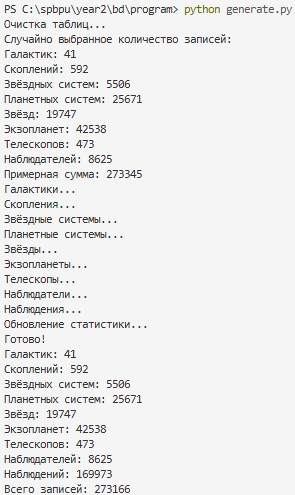
\includegraphics[width=0.7\linewidth]{generation}
		\caption{Заполнение таблицы в консоли.}
		\label{generation}
	\end{figure}

Как видно на рис. \ref{generation}, в таблице содержится 273~166 записей.

Полный текст программы генерации тестовых данных приведён в разделе \hyperref[b][Приложение Б].

\subsection{Запросы}

Для измерения времени запросов предварительно была выполнена команда \texttt{\textbackslash{}timing}.

\subsubsection{Запрос 1}

Запрос: "Найти все телескопы, которые наблюдали тип экзопланет A в галактике B вокруг звёзд класса C".

Были выбраны следующие поля для поиска:

\begin{itemize}
  \item A --- terrestrial;
  \item B --- GAL\_0001;
  \item C --- G.
\end{itemize}

Текст запроса на SQL приведён в листинге \ref{lst:q1t}.

\begin{lstlisting}[language=SQL, caption={Текст запроса №1}, label={lst:q1t}]
SELECT
    t.tele_id,
    t.tele_type,
    t.aper,
    t.com_year,
    t.oper,
    t.discov_plan
FROM telescope t
JOIN observation o
    ON o.tele_id = t.tele_id
JOIN exoplanet e
    ON e.exo_id = o.exo_id
JOIN plan_system ps
    ON ps.system_id = e.sys_id
JOIN star s
    ON s.sys_id = ps.system_id
JOIN stellar_system ss
    ON ss.stellar_id = ps.stell_sys_id
JOIN cluster c
    ON c.cluster_id = ss.cluster_id
JOIN galaxy g
    ON g.galaxy_id = c.galaxy_id
WHERE e.exo_type = 'terrestrial'
  AND g.galaxy_id = 'GAL_0001'
  AND s.class = 'G'
GROUP BY
    t.tele_id,
    t.tele_type,
    t.aper,
    t.com_year,
    t.oper,
    t.discov_plan
ORDER BY t.tele_id;
\end{lstlisting}

Реляционная формула запроса:

\[
\begin{aligned}
&\tau_{\mathrm{tele_id}}\Big(\
&\quad \gamma_{\mathrm{tele_id, tele_type, aper, com_year, oper, discov_plan;}}\Big(\
&\quad\quad \sigma_{\mathrm{exo_type = terrestrial \land galaxy_id = GAL_0001 \land class = G}}\Big(\
&\quad\quad\quad \mathrm{telescope}\
&\quad\quad\quad \bowtie_{\mathrm{tele_id}} \mathrm{observation}\
&\quad\quad\quad \bowtie_{\mathrm{exo_id}} \mathrm{exoplanet}\
&\quad\quad\quad \bowtie_{\mathrm{sys_id}} \mathrm{plan_system}\
&\quad\quad\quad \bowtie_{\mathrm{sys_id}} \mathrm{star}\
&\quad\quad\quad \bowtie_{\mathrm{stellar_id}} \mathrm{stellar_system}\
&\quad\quad\quad \bowtie_{\mathrm{cluster_id}} \mathrm{cluster}\
&\quad\quad\quad \bowtie_{\mathrm{galaxy_id}} \mathrm{galaxy}\
&\quad\quad\Big)\
&\quad\Big)\
&\Big)
\end{aligned}
\]

Последовательность выполнения запроса приведена в табл. \ref{tab:q1plan}.

\begin{table}[H]
	\centering
	\caption{Последовательность выполнения запроса 1}
	\label{tab:q1plan}
	\small
	\begin{tabularx}{\linewidth}{>{\centering\arraybackslash}p{0.9cm}>{\RaggedRight\arraybackslash}p{4.1cm}X}
		\toprule
		Шаг & Операция & Описание \\
		\midrule
		1 & Scan & Чтение таблиц телескопов, наблюдений, экзопланет, планетарных систем, звёзд, звёздных систем, скоплений и галактик. \\
		2 & Join & Соединение наблюдений с телескопами и экзопланетами. \\
		3 & Join & Переход от экзопланет к планетарным системам, звёздам, звёздным системам, скоплениям и галактикам. \\
		4 & Filter & Отбор записей с типом экзопланеты terrestrial, галактикой GAL\_0001 и классом звезды G. \\
		5 & GroupAggregate & Группировка по телескопу и подсчёт различных наблюдений и экзопланет. \\
		6 & Sort & Сортировка результата по идентификатору телескопа. \\
		\bottomrule
	\end{tabularx}
\end{table}

Планировщик строит цепочку соединений от наблюдений к астрономическим объектам и применяет фильтры по типу экзопланеты, галактике и классу звезды. После этого строки группируются по телескопам, для каждой группы вычисляется количество различных наблюдений и экзопланет, затем результат сортируется по идентификатору телескопа.

Фрагмент результата выполнения первого запроса приведён на рис. \ref{q1r}.

\begin{figure}[H]
	\centering
	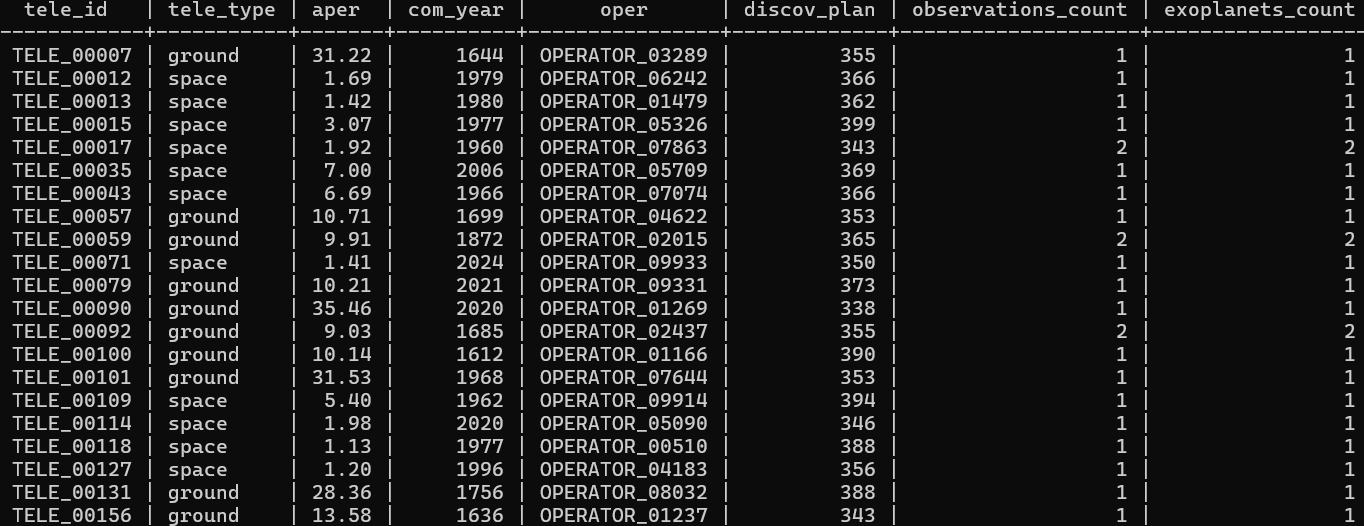
\includegraphics[width=0.85\linewidth]{images/queries/q1r.png}
	\caption{Фрагмент результата выполнения первого запроса.}
	\label{q1r}
\end{figure}

Время выполнения запроса: 19.875 мс.

\subsubsection{Запрос 2}

Запрос: Для наблюдателя A посчитать число звёзд, которые он наблюдал в типе телескопа B.

Были выбраны следующие поля для поиска:

\begin{itemize}
  \item A --- Observer\_000001;
  \item B --- ground.
\end{itemize}

Текст запроса на SQL приведён в листинге \ref{lst:q2t}.

\begin{lstlisting}[language=SQL, caption={Текст запроса №2}, label={lst:q2t}]
SELECT
    o.observer_id,
    t.tele_type,
    COUNT(DISTINCT s.star_id) AS stars_count
FROM observation o
JOIN telescope t
    ON t.tele_id = o.tele_id
JOIN exoplanet e
    ON e.exo_id = o.exo_id
JOIN plan_system ps
    ON ps.system_id = e.sys_id
JOIN star s
    ON s.sys_id = ps.system_id
WHERE o.observer_id = 'Observer_000001'
  AND t.tele_type = 'ground'
GROUP BY o.observer_id, t.tele_type;
\end{lstlisting}

Реляционная формула запроса:

\[
\begin{aligned}
&\gamma_{\mathrm{observer_id, tele_type; COUNTD(star_id)}}\Big(\
&\quad \sigma_{\mathrm{observer_id = Observer_000001 \land tele_type = ground}}\Big(\
&\quad\quad \mathrm{observation}\
&\quad\quad \bowtie_{\mathrm{tele_id}} \mathrm{telescope}\
&\quad\quad \bowtie_{\mathrm{exo_id}} \mathrm{exoplanet}\
&\quad\quad \bowtie_{\mathrm{sys_id}} \mathrm{plan_system}\
&\quad\quad \bowtie_{\mathrm{sys_id}} \mathrm{star}\
&\quad\quad \Big)\
&\Big)
\end{aligned}
\]


Последовательность выполнения запроса приведена в табл. \ref{tab:q2plan}.

\begin{table}[H]
	\centering
	\caption{Последовательность выполнения запроса 2}
	\label{tab:q2plan}
	\small
	\begin{tabularx}{\linewidth}{>{\centering\arraybackslash}p{0.9cm}>{\RaggedRight\arraybackslash}p{4.1cm}X}
		\toprule
		Шаг & Операция & Описание \\
		\midrule
		1 & Filter & Отбор наблюдений, выполненных наблюдателем Observer\_000001. \\
		2 & Join & Соединение наблюдений с телескопами. \\
		3 & Filter & Отбор телескопов типа ground. \\
		4 & Join & Соединение с экзопланетами, планетарными системами и звёздами. \\
		5 & GroupAggregate & Группировка по наблюдателю и типу телескопа, подсчёт различных звёзд. \\
		\bottomrule
	\end{tabularx}
\end{table}

Сначала выбираются наблюдения нужного наблюдателя, после чего они связываются с телескопами и ограничиваются наземным типом. Затем через экзопланету и планетарную систему определяется множество звёзд, а агрегирование считает количество различных звёзд в найденной группе.

Фрагмент результата выполнения второго запроса приведён на рис. \ref{q2r}.
\begin{figure}[H]
	\centering
	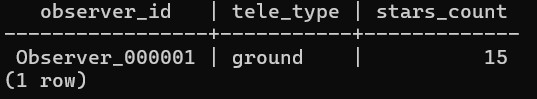
\includegraphics[width=0.85\linewidth]{images/queries/q2r.png}
	\caption{Фрагмент результата выполнения второго запроса.}
	\label{q2r}
\end{figure}


Время выполнения запроса: 54.028 мс.

\subsubsection{Запрос 3}

Запрос: Для каждого класса звезды посчитать число звёзд и число наблюдений, построить 2D-гистограмму.

Данный запрос выполняется по всем классам звёзд, поэтому дополнительные поля для поиска не выбирались.

Текст запроса на SQL приведён в листинге \ref{lst:q3t}.

\begin{lstlisting}[language=SQL, caption={Текст запроса №3}, label={lst:q3t}]
SELECT
    s.class AS star_class,
    COUNT(DISTINCT s.star_id) AS stars_count,
    COUNT(DISTINCT o.observation_id) AS observations_count
FROM star s
JOIN plan_system ps
    ON ps.system_id = s.sys_id
JOIN exoplanet e
    ON e.sys_id = ps.system_id
JOIN observation o
    ON o.exo_id = e.exo_id
GROUP BY s.class
ORDER BY s.class;
\end{lstlisting}

Реляционная формула запроса:

\[
\begin{aligned}
&\tau_{\mathrm{class}}\Big(\
&\quad \gamma_{\mathrm{class; COUNTD(star_id), COUNTD(observation_id)}}\Big(\
&\quad\quad \mathrm{star}\
&\quad\quad \mathbin{\operatorname{LEFTJOIN}}*{\mathrm{sys_id}} \mathrm{plan_system}\
&\quad\quad \mathbin{\operatorname{LEFTJOIN}}*{\mathrm{system_id = sys_id}} \mathrm{exoplanet}\
&\quad\quad \mathbin{\operatorname{LEFTJOIN}}_{\mathrm{exo_id}} \mathrm{observation}\
&\quad\quad \Big)\
&\Big)
\end{aligned}
\]


Последовательность выполнения запроса приведена в табл. \ref{tab:q3plan}.

\begin{table}[H]
	\centering
	\caption{Последовательность выполнения запроса 3}
	\label{tab:q3plan}
	\small
	\begin{tabularx}{\linewidth}{>{\centering\arraybackslash}p{0.9cm}>{\RaggedRight\arraybackslash}p{4.1cm}X}
		\toprule
		Шаг & Операция & Описание \\
		\midrule
		1 & Scan & Чтение таблицы звёзд. \\
		2 & Left Join & Присоединение планетарных систем к звёздам. \\
		3 & Left Join & Присоединение экзопланет к планетарным системам. \\
		4 & Left Join & Присоединение наблюдений к экзопланетам. \\
		5 & GroupAggregate & Группировка по классу звезды, подсчёт звёзд и наблюдений. \\
		6 & Sort & Сортировка классов звёзд. \\
		\bottomrule
	\end{tabularx}
\end{table}

Запрос начинает выполнение с таблицы звёзд, поэтому классы без наблюдений не теряются. Внешние соединения добавляют связанные планетарные системы, экзопланеты и наблюдения, после чего агрегирование считает число различных звёзд и наблюдений для каждого класса.

Фрагмент результата выполнения третьего запроса приведён на рис. \ref{q3r}.

\begin{figure}[H]
	\centering
	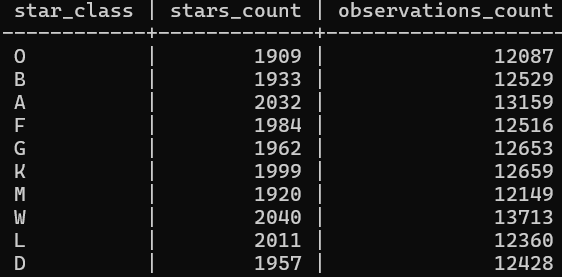
\includegraphics[width=0.85\linewidth]{images/queries/q3r.png}
	\caption{Фрагмент результата выполнения третьего запроса.}
	\label{q3r}
\end{figure}

Гистограмма результата изображена на рис. \ref{q3h}:

\begin{figure}[H]
	\centering
	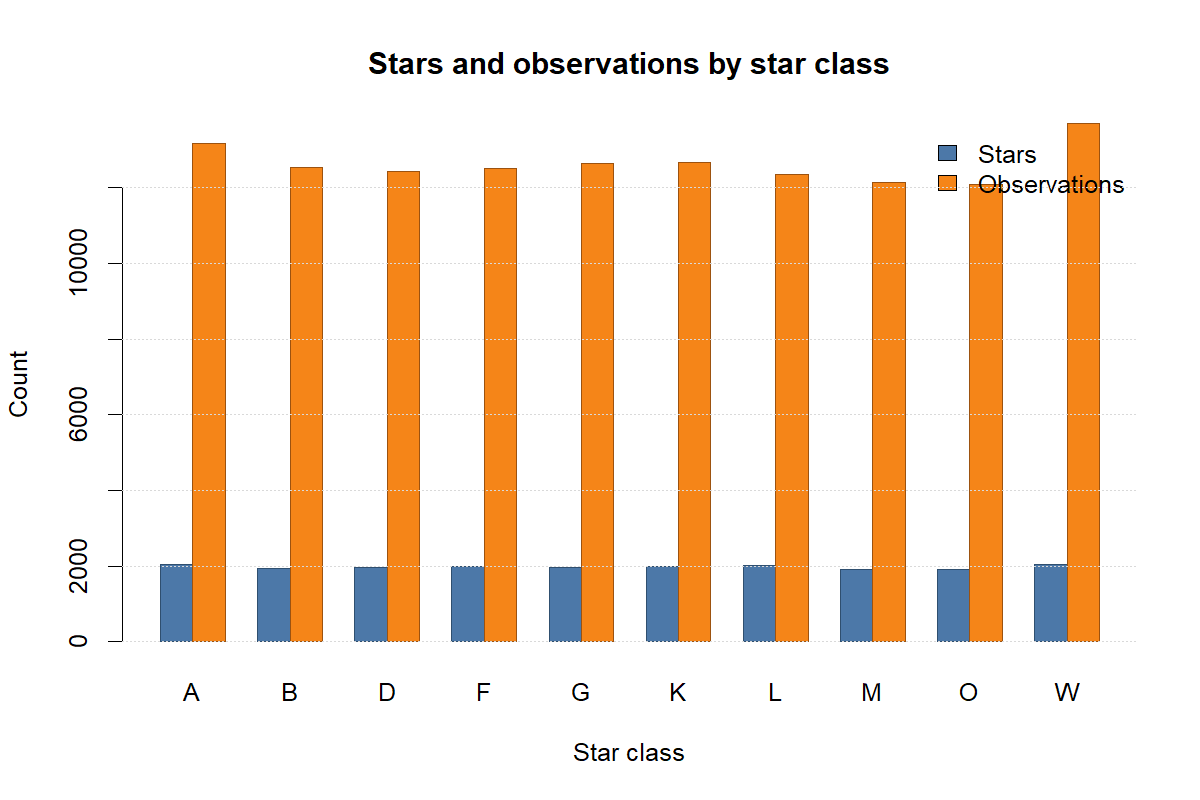
\includegraphics[width=0.85\linewidth]{images/queries/q3h.png}
	\caption{Гистограмма результата выполнения третьего запроса.}
	\label{q3h}
\end{figure}

Время выполнения запроса: 724.394 мс.

\subsubsection{Запрос 4.1}

Запрос: Найти страны, из которых наблюдалось максимальное число экзопланет.

Данный запрос выполняется по всем странам наблюдателей, поэтому дополнительные поля для поиска не выбирались.

Текст запроса на SQL приведён в листинге \ref{lst:q41t}.

\begin{lstlisting}[language=SQL, caption={Текст запроса №4.1}, label={lst:q41t}]
SELECT country, exoplanets_count
FROM (
    SELECT
        obs.country,
        COUNT(DISTINCT o.exo_id) AS exoplanets_count
    FROM observer obs
    JOIN observation o ON o.observer_id = obs.observer_id
    GROUP BY obs.country
)
WHERE exoplanets_count = (
    SELECT MAX(exoplanets_count)
    FROM (
        SELECT COUNT(DISTINCT o2.exo_id) AS exoplanets_count
        FROM observation o2
        JOIN observer obs2 ON obs2.observer_id = o2.observer_id
        GROUP BY obs2.country
    )
)
ORDER BY exoplanets_count DESC;
\end{lstlisting}

Реляционная формула запроса:

\[
\begin{aligned}
&\tau_{\mathrm{exoplanets\_count} \downarrow}\Bigg( \\
&\quad \pi_{\mathrm{country},\, \mathrm{exoplanets\_count}}\Bigg( \\
&\quad\quad \sigma_{\mathrm{exoplanets\_count} \geq \mathrm{all\_other\_counts}}\Bigg( \\
&\quad\quad\quad \rho_{\mathrm{temp}}(\gamma_{\mathrm{country};\, \text{COUNTD}(\mathrm{exo\_id}) \to \mathrm{exoplanets\_count}}(\mathrm{observer} \bowtie_{\mathrm{observer\_id}} \mathrm{observation})) \\
&\quad\quad \Bigg) \\
&\quad \Bigg) \\
&\Bigg)
\end{aligned}
\]

Последовательность выполнения запроса приведена в табл. \ref{tab:q41plan}.

\begin{table}[H]
	\centering
	\caption{Последовательность выполнения запроса 4.1}
	\label{tab:q41plan}
	\small
	\begin{tabularx}{\linewidth}{>{\centering\arraybackslash}p{0.9cm}>{\RaggedRight\arraybackslash}p{4.1cm}X}
		\toprule
		Шаг & Операция & Описание \\
		\midrule
		1 & Scan & Чтение наблюдателей и наблюдений. \\
		2 & Join & Соединение наблюдений со странами наблюдателей. \\
		3 & GroupAggregate & Группировка по стране и подсчёт различных экзопланет. \\
		4 & Sort & Сортировка стран по убыванию числа экзопланет. \\
		5 & Fetch First With Ties & Выбор страны или стран с максимальным значением. \\
		\bottomrule
	\end{tabularx}
\end{table}

Запрос связывает каждое наблюдение со страной наблюдателя, затем считает количество различных экзопланет для каждой страны. После сортировки по убыванию выбирается верхняя строка вместе со всеми строками, имеющими такое же максимальное значение.

Фрагмент результата выполнения запроса 4.1 приведён на рис. \ref{q41r}.

\begin{figure}[H]
	\centering
	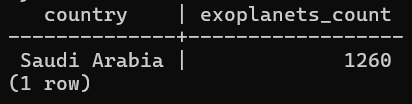
\includegraphics[width=0.85\linewidth]{images/queries/q41r.png}
	\caption{Фрагмент результата выполнения запроса 4.1.}
	\label{q41r}
\end{figure}

Время выполнения запроса: 1106.565 мс.

\subsubsection{Запрос 4.2}

Запрос: Найти страны, из которых наблюдалось минимальное число экзопланет.

Данный запрос выполняется по всем странам наблюдателей, поэтому дополнительные поля для поиска не выбирались.

Текст запроса на SQL приведён в листинге \ref{lst:q42t}.

\begin{lstlisting}[language=SQL, caption={Текст запроса №4.2}, label={lst:q42t}]
SELECT country, exoplanets_count
FROM (
    SELECT
        obs.country,
        COUNT(DISTINCT o.exo_id) AS exoplanets_count
    FROM observer obs
    JOIN observation o ON o.observer_id = obs.observer_id
    GROUP BY obs.country
)
WHERE exoplanets_count = (
    SELECT MIN(exoplanets_count)
    FROM (
        SELECT COUNT(DISTINCT o2.exo_id) AS exoplanets_count
        FROM observation o2
        JOIN observer obs2 ON obs2.observer_id = o2.observer_id
        GROUP BY obs2.country
    )
)
ORDER BY exoplanets_count DESC;
\end{lstlisting}

Реляционная формула запроса:

\[
\begin{aligned}
&\lambda_{1}^{\mathrm{ties}}\Big(\\
&\quad \tau_{\mathrm{exoplanets_count}\uparrow}\Big(\\
&\quad\quad \gamma_{\mathrm{country; COUNTD(exo_id) \rightarrow exoplanets_count}}\Big(\\
&\quad\quad\quad \mathrm{observer}\\
&\quad\quad\quad \bowtie_{\mathrm{observer_id}} \mathrm{observation}\\
&\quad\quad\Big)\\
&\quad\Big)\\
&\Big)
\end{aligned}
\]


Последовательность выполнения запроса приведена в табл. \ref{tab:q42plan}.

\begin{table}[H]
	\centering
	\caption{Последовательность выполнения запроса 4.2}
	\label{tab:q42plan}
	\small
	\begin{tabularx}{\linewidth}{>{\centering\arraybackslash}p{0.9cm}>{\RaggedRight\arraybackslash}p{4.1cm}X}
		\toprule
		Шаг & Операция & Описание \\
		\midrule
		1 & Scan & Чтение наблюдателей и наблюдений. \\
		2 & Join & Соединение наблюдений со странами наблюдателей. \\
		3 & GroupAggregate & Группировка по стране и подсчёт различных экзопланет. \\
		4 & Sort & Сортировка стран по возрастанию числа экзопланет. \\
		5 & Fetch First With Ties & Выбор страны или стран с минимальным значением. \\
		\bottomrule
	\end{tabularx}
\end{table}

Фрагмент результата выполнения запроса 4.2 приведён на рис. \ref{q42r}.

\begin{figure}[H]
	\centering
	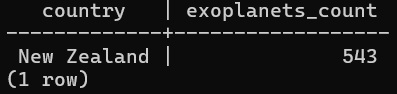
\includegraphics[width=0.85\linewidth]{images/queries/q42r.png}
	\caption{Фрагмент результата выполнения запроса 4.2.}
	\label{q42r}
\end{figure}

Время выполнения запроса: 1102.927 мс.

\subsubsection{Запрос 5}

Запрос: Посчитать число экзопланет с равным числом наблюдений, построить 2D-гистограмму.

Данный запрос выполняется по всем экзопланетам, поэтому дополнительные поля для поиска не выбирались.

Текст запроса на SQL приведён в листинге \ref{lst:q5t}.

\begin{lstlisting}[language=SQL, caption={Текст запроса №5}, label={lst:q5t}]
SELECT
    observations_count,
    COUNT(*) AS exoplanets_count
FROM (
    SELECT
        e.exo_id,
        COUNT(o.observation_id) AS observations_count
    FROM exoplanet e
    JOIN observation o
        ON o.exo_id = e.exo_id
    GROUP BY e.exo_id
) AS exoplanet_observations 
GROUP BY observations_count
ORDER BY observations_count;
\end{lstlisting}

Реляционная формула запроса:

\[
\begin{aligned}
&\tau_{\mathrm{observations_count}}\Big(\\
&\quad \gamma_{\mathrm{observations_count; COUNT(*) \rightarrow exoplanets_count}}\Big(\\
&\quad\quad \gamma_{\mathrm{exo_id; COUNT(observation_id) \rightarrow observations_count}}\Big(\\
&\quad\quad\quad \mathrm{exoplanet}\\
&\quad\quad\quad \mathbin{\operatorname{LEFTJOIN}}_{\mathrm{exo_id}} \mathrm{observation}\\
&\quad\quad\Big)\\
&\quad\Big)\\
&\Big)
\end{aligned}
\]

Последовательность выполнения запроса приведена в табл. \ref{tab:q5plan}.

\begin{table}[H]
	\centering
	\caption{Последовательность выполнения запроса 5}
	\label{tab:q5plan}
	\small
	\begin{tabularx}{\linewidth}{>{\centering\arraybackslash}p{0.9cm}>{\RaggedRight\arraybackslash}p{4.1cm}X}
		\toprule
		Шаг & Операция & Описание \\
		\midrule
		1 & Scan & Чтение экзопланет и наблюдений. \\
		2 & Left Join & Присоединение наблюдений к каждой экзопланете, включая экзопланеты без наблюдений. \\
		3 & GroupAggregate & Подсчёт числа наблюдений для каждой экзопланеты. \\
		4 & GroupAggregate & Подсчёт количества экзопланет для каждого полученного числа наблюдений. \\
		5 & Sort & Сортировка результата по числу наблюдений. \\
		\bottomrule
	\end{tabularx}
\end{table}

Запрос выполняет агрегирование в два уровня. Сначала для каждой экзопланеты считается число связанных наблюдений, затем результат группируется повторно, чтобы определить, сколько экзопланет имеют одинаковое количество наблюдений.

Фрагмент результата выполнения пятого запроса приведён на рис. \ref{q5r}.

\begin{figure}[H]
	\centering
	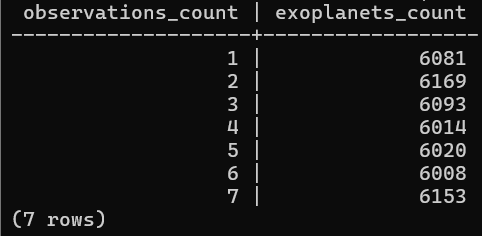
\includegraphics[width=0.85\linewidth]{images/queries/q5r.png}
	\caption{Фрагмент результата выполнения пятого запроса.}
	\label{q5r}
\end{figure}

Гистограмма результата изображена на рис. \ref{q5h}:

\begin{figure}[H]
	\centering
	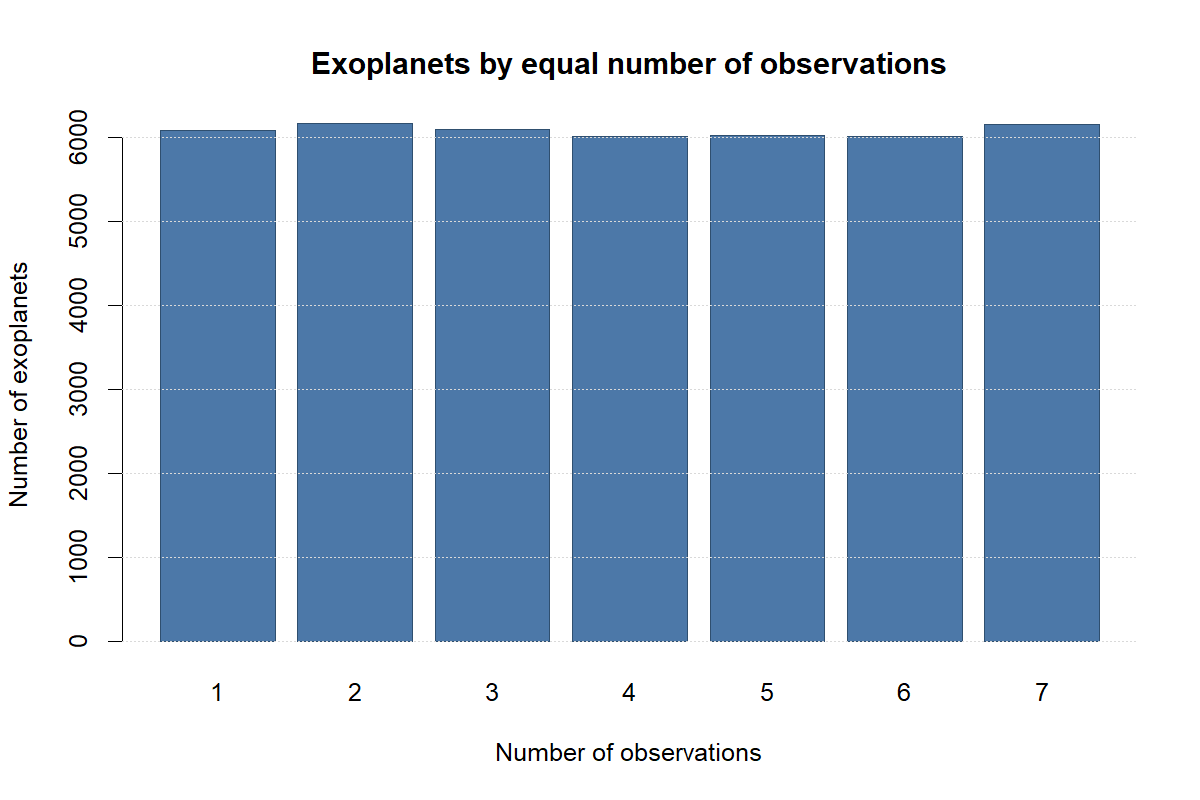
\includegraphics[width=0.85\linewidth]{images/queries/q5h.png}
	\caption{Гистограмма результата выполнения пятого запроса.}
	\label{q5h}
\end{figure}

Время выполнения запроса: 76.010 мс.

\subsubsection{Запрос 6}

Запрос: Найти галактику, в которой не наблюдалось ни одной звезды выбранным типом телескопа.

Было выбрано следующее поле для поиска:

\begin{itemize}
  \item A --- ground.
\end{itemize}

Текст запроса на SQL приведён в листинге \ref{lst:q6t}.

\begin{lstlisting}[language=SQL, caption={Текст запроса №6}, label={lst:q6t}]
SELECT g.galaxy_id
FROM galaxy g
WHERE NOT EXISTS (
    SELECT 1
    FROM cluster c
    JOIN stellar_system s ON s.cluster_id = c.cluster_id
    JOIN plan_system ps ON ps.stell_sys_id = s.stellar_id
    JOIN exoplanet e ON e.sys_id = ps.system_id
    JOIN observation o ON o.exo_id = e.exo_id
    JOIN telescope t ON t.tele_id = o.tele_id
    WHERE c.galaxy_id = g.galaxy_id
      AND t.tele_type = 'ground'
);
\end{lstlisting}

Реляционная формула запроса:

\[
\begin{aligned}
&\tau_{\mathrm{galaxy_id}}\Big(\\
&\quad \sigma_{\mathrm{observed_stars_count} = 0}\Big(\\
&\quad\quad \gamma_{\mathrm{galaxy_id, conf_plan, hab_plan, dist; COUNTD(star_id) \rightarrow observed_stars_count}}\Big(\\
&\quad\quad\quad \mathrm{galaxy}\\
&\quad\quad\quad \mathbin{\operatorname{LEFTJOIN}}*{\mathrm{galaxy_id}} \mathrm{cluster}\\
&\quad\quad\quad \mathbin{\operatorname{LEFTJOIN}}*{\mathrm{cluster_id}} \mathrm{stellar_system}\\
&\quad\quad\quad \mathbin{\operatorname{LEFTJOIN}}*{\mathrm{stellar_id} = \mathrm{stell_sys_id}} \mathrm{plan_system}\\
&\quad\quad\quad \mathbin{\operatorname{LEFTJOIN}}*{\mathrm{system_id} = \mathrm{sys_id}} \mathrm{star}\\
&\quad\quad\quad \mathbin{\operatorname{LEFTJOIN}}*{\mathrm{system_id} = \mathrm{sys_id}} \mathrm{exoplanet}\\
&\quad\quad\quad \mathbin{\operatorname{LEFTJOIN}}*{\mathrm{exo_id}} \mathrm{observation}\\
&\quad\quad\quad \mathbin{\operatorname{LEFTJOIN}}_{\mathrm{tele_id} \land \mathrm{tele_type} = \mathrm{ground}} \mathrm{telescope}\\
&\quad\quad\Big)\\
&\quad\Big)\\
&\Big)
\end{aligned}
\]

Последовательность выполнения запроса приведена в табл. \ref{tab:q6plan}.

\begin{table}[H]
	\centering
	\caption{Последовательность выполнения запроса 6}
	\label{tab:q6plan}
	\small
	\begin{tabularx}{\linewidth}{>{\centering\arraybackslash}p{0.9cm}>{\RaggedRight\arraybackslash}p{4.1cm}X}
		\toprule
		Шаг & Операция & Описание \\
		\midrule
		1 & Scan & Чтение таблицы галактик. \\
		2 & Left Join & Присоединение скоплений, звёздных систем, планетарных систем и звёзд. \\
		3 & Left Join & Присоединение экзопланет и наблюдений. \\
		4 & Left Join + Filter & Присоединение только наземных телескопов. \\
		5 & GroupAggregate & Группировка по галактикам и подсчёт различных наблюдавшихся звёзд. \\
		6 & Having & Отбор галактик, где число таких звёзд равно нулю. \\
		7 & Sort & Сортировка результата по идентификатору галактики. \\
		\bottomrule
	\end{tabularx}
\end{table}

Запрос сохраняет все галактики за счёт внешних соединений, а затем постепенно присоединяет связанные уровни иерархии. Условие на тип телескопа применяется при соединении с таблицей телескопов, поэтому агрегирование считает только звёзды, наблюдавшиеся через наземные телескопы; оператор \texttt{HAVING} оставляет галактики с нулевым количеством таких звёзд.

Фрагмент результата выполнения шестого запроса приведён на рис. \ref{q6r}.

\begin{figure}[H]
	\centering
	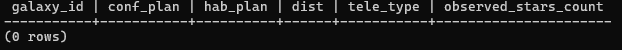
\includegraphics[width=0.85\linewidth]{images/queries/q6r.png}
	\caption{Фрагмент результата выполнения шестого запроса.}
	\label{q6r}
\end{figure}

Время выполнения запроса: 114.952 мс.

\subsubsection{Запрос 7}

Запрос: Найти наблюдателей, которые наблюдали больше экзопланет, чем наблюдатель A.

Было выбрано следующее поле для поиска:

\begin{itemize}
  \item A --- Observer\_000001.
\end{itemize}

Текст запроса на SQL приведён в листинге \ref{lst:q7t}.

\begin{lstlisting}[language=SQL, caption={Текст запроса №7}, label={lst:q7t}]
SELECT
    obs.observer_id,
    obs.country,
    COUNT(DISTINCT o.exo_id) AS exoplanets_count
FROM observer obs
JOIN observation o ON o.observer_id = obs.observer_id
GROUP BY obs.observer_id, obs.country
HAVING COUNT(DISTINCT o.exo_id) > (
    SELECT COUNT(DISTINCT o2.exo_id)
    FROM observer obs2
    JOIN observation o2 ON o2.observer_id = obs2.observer_id
    WHERE obs2.observer_id = 'Observer_0000001'
)
ORDER BY COUNT(DISTINCT o.exo_id) DESC, obs.observer_id;
\end{lstlisting}

Реляционная формула запроса:

\[
\begin{aligned}
&\tau_{\mathrm{exoplanets_count}\downarrow, \mathrm{observer_id}}\Big(\
&\quad \sigma_{\mathrm{observer_id} \neq \mathrm{target.observer_id} \land \mathrm{exoplanets_count} > \mathrm{target.exoplanets_count}}\Big(\
&\quad\quad \gamma_{\mathrm{observer_id, country; COUNTD(exo_id) \rightarrow exoplanets_count}}\Big(\
&\quad\quad\quad \mathrm{observer}\
&\quad\quad\quad \mathbin{\operatorname{LEFTJOIN}}*{\mathrm{observer_id}} \mathrm{observation}\
&\quad\quad\Big)\
&\quad\quad \bowtie*{\mathrm{target.observer_id} = \mathrm{Observer_000001}} , \rho_{\mathrm{target}}\Big(\
&\quad\quad\quad \gamma_{\mathrm{observer_id, country; COUNTD(exo_id) \rightarrow exoplanets_count}}\Big(\
&\quad\quad\quad\quad \mathrm{observer}\
&\quad\quad\quad\quad \mathbin{\operatorname{LEFTJOIN}}_{\mathrm{observer_id}} \mathrm{observation}\
&\quad\quad\quad\Big)\
&\quad\quad\Big)\
&\Big)\Big)
\end{aligned}
\]


Последовательность выполнения запроса приведена в табл. \ref{tab:q7plan}.

\begin{table}[H]
	\centering
	\caption{Последовательность выполнения запроса 7}
	\label{tab:q7plan}
	\small
	\begin{tabularx}{\linewidth}{>{\centering\arraybackslash}p{0.9cm}>{\RaggedRight\arraybackslash}p{4.1cm}X}
		\toprule
		Шаг & Операция & Описание \\
		\midrule
		1 & Materialized CTE & Формирование временного набора observer\_counts. \\
		2 & Left Join & Присоединение наблюдений к каждому наблюдателю. \\
		3 & GroupAggregate & Подсчёт различных экзопланет для каждого наблюдателя. \\
		4 & Filter & Выбор строки целевого наблюдателя Observer\_000001. \\
		5 & Join + Filter & Сравнение всех наблюдателей с целевым и отбор тех, у кого экзопланет больше. \\
		6 & Sort & Сортировка по убыванию числа экзопланет и идентификатору наблюдателя. \\
		\bottomrule
	\end{tabularx}
\end{table}

Сначала материализуется вспомогательный набор с количеством различных экзопланет для каждого наблюдателя. Затем из него выбирается целевой наблюдатель, после чего остальные строки сравниваются с его значением; в результат попадают только наблюдатели с большим числом наблюдавшихся экзопланет.

Фрагмент результата выполнения седьмого запроса приведён на рис. \ref{q7r}.

\begin{figure}[H]
	\centering
	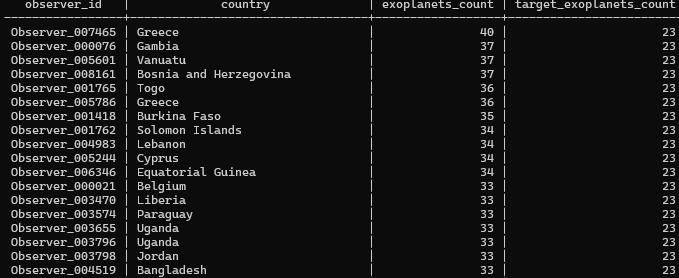
\includegraphics[width=0.85\linewidth]{images/queries/q7r.png}
	\caption{Фрагмент результата выполнения седьмого запроса.}
	\label{q7r}
\end{figure}

Время выполнения запроса: 177.400 мс.

\subsubsection{Запрос 8}

Запрос: Для каждого телескопа и для каждой страны посчитать число наблюдений, построить 3D-гистограмму.

Данный запрос выполняется по всем телескопам и странам, поэтому дополнительные поля для поиска не выбирались.

Текст запроса на SQL приведён в листинге \ref{lst:q8t}.

\begin{lstlisting}[language=SQL, caption={Текст запроса №8}, label={lst:q8t}]
SELECT t.tele_id, c.country, COUNT(o.observation_id)
FROM
    (SELECT tele_id
     FROM telescope
     ORDER BY tele_id
     LIMIT 20) t
CROSS JOIN
    (SELECT DISTINCT country
     FROM observer
     ORDER BY country
     LIMIT 20) c
JOIN observer ob
    ON ob.country = c.country
JOIN observation o
    ON o.observer_id = ob.observer_id
   AND o.tele_id = t.tele_id
GROUP BY t.tele_id, c.country
ORDER BY t.tele_id, c.country;
\end{lstlisting}

Реляционная формула запроса:

\[
\begin{aligned}
&\tau_{\mathrm{observations_count}\downarrow, \mathrm{tele_id}, \mathrm{country}}\Big(\
&\quad \big(\mathrm{telescope} \times \operatorname{enum_range}(\mathrm{country_enum})\big)\
&\quad \mathbin{\operatorname{LEFTJOIN}}*{\mathrm{tele_id, country}}
\gamma*{\mathrm{tele_id, country; COUNT(*) \rightarrow observations_count}}\Big(\
&\quad\quad \mathrm{observation}\
&\quad\quad \bowtie_{\mathrm{observer_id}} \mathrm{observer}\
&\quad\Big)\
&\Big)
\end{aligned}
\]


Последовательность выполнения запроса приведена в табл. \ref{tab:q8plan}.

\begin{table}[H]
	\centering
	\caption{Последовательность выполнения запроса 8}
	\label{tab:q8plan}
	\small
	\begin{tabularx}{\linewidth}{>{\centering\arraybackslash}p{0.9cm}>{\RaggedRight\arraybackslash}p{4.1cm}X}
		\toprule
		Шаг & Операция & Описание \\
		\midrule
		1 & Materialized CTE & Формирование набора observed\_counts. \\
		2 & Join & Соединение наблюдений с наблюдателями для получения страны. \\
		3 & GroupAggregate & Подсчёт числа наблюдений для каждой пары телескоп--страна. \\
		4 & Cross Join & Построение всех комбинаций телескопов и стран из перечисления country\_enum. \\
		5 & Left Join & Присоединение фактических количеств наблюдений к полному набору комбинаций. \\
		6 & Projection & Замена отсутствующих значений на 0 с помощью \texttt{COALESCE}. \\
		7 & Sort & Сортировка по убыванию числа наблюдений, телескопу и стране. \\
		\bottomrule
	\end{tabularx}
\end{table}

Вспомогательный набор сначала считает реальные наблюдения по парам телескоп--страна. Затем \texttt{CROSS JOIN} создаёт полный набор возможных пар из всех телескопов и всех стран, после чего внешнее соединение добавляет рассчитанные значения; для отсутствующих наблюдений используется ноль.

Фрагмент результата выполнения восьмого запроса приведён на рис. \ref{q8r}.

\begin{figure}[H]
	\centering
	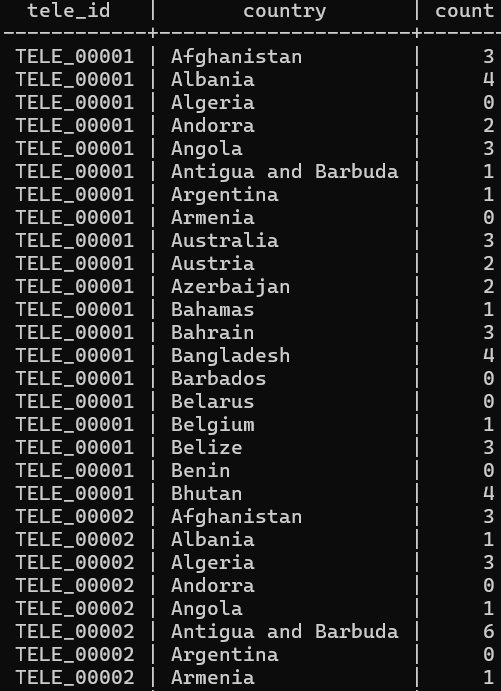
\includegraphics[width=0.85\linewidth]{images/queries/q8r.png}
	\caption{Фрагмент результата выполнения восьмого запроса.}
	\label{q8r}
\end{figure}

Гистограмма результата для топ-20 изображена на рис. \ref{q8h}:

\begin{figure}[H]
	\centering
	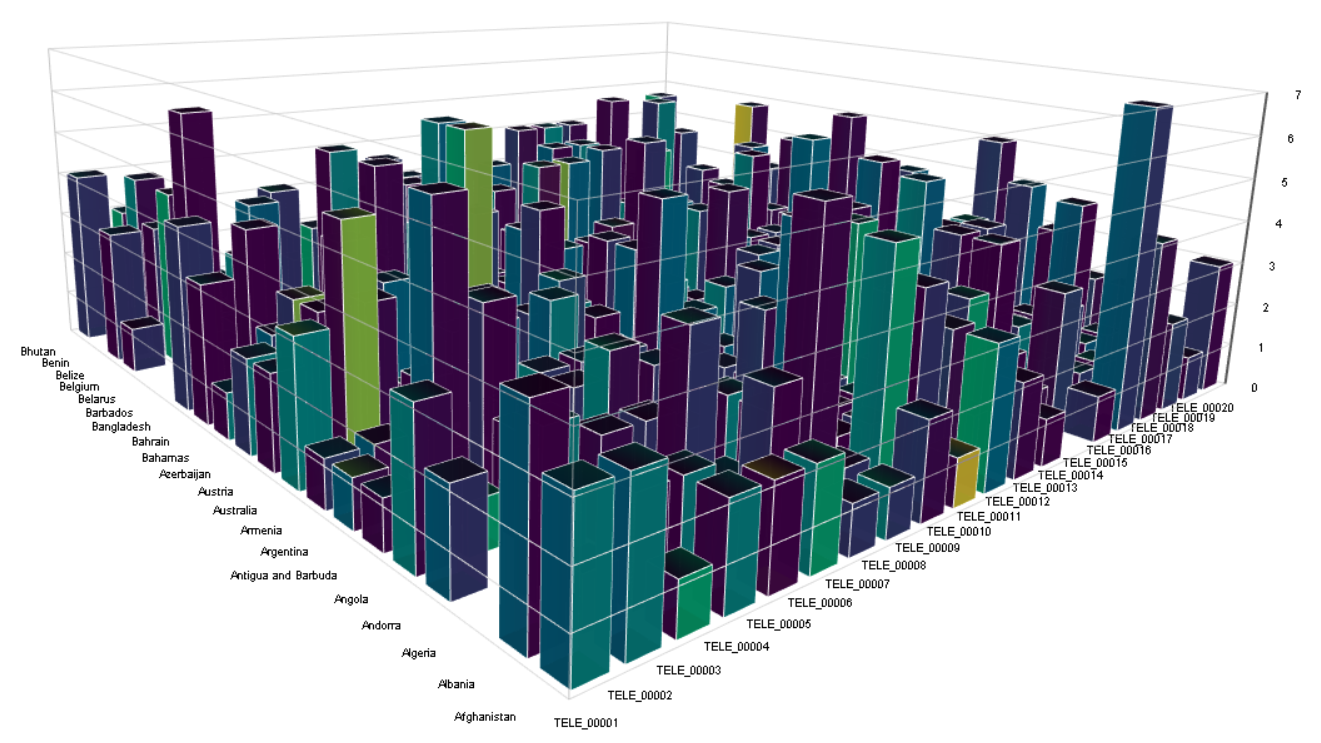
\includegraphics[width=1\linewidth]{images/queries/q8h.png}
	\caption{Гистограмма результата выполнения восьмого запроса.}
	\label{q8h}
\end{figure}

Время выполнения запроса: 42.186 мс.

\subsubsection{Запрос 9}

Запрос: Для всех наблюдений через телескоп A, в которых наблюдается объект B, поменять наблюдения на наблюдения для наблюдателя C.

Перед выполнением запроса был введён следующий запрос, чтобы найти такие телескопы, из которых одна экзопланета наблюдалась более 1 раза (листинг \ref{lst:q9prep}):

\begin{lstlisting}[language=SQL, caption={Подготовка к девятому запросу.}, label={lst:q9prep}]
SELECT
    tele_id,
    exo_id,
    COUNT(*) AS observations_count
FROM observation
GROUP BY tele_id, exo_id
HAVING COUNT(*) > 1
ORDER BY observations_count DESC, tele_id, exo_id
LIMIT 20;
\end{lstlisting}

Результат изображён на рис. \ref{q9prep}.

\begin{figure}[H]
	\centering
	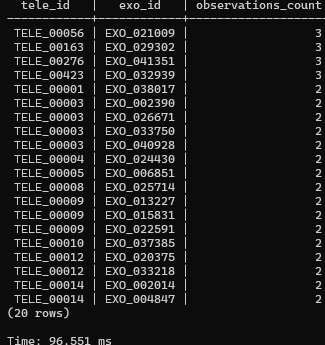
\includegraphics[width=0.85\linewidth]{images/queries/q9prep.png}
	\caption{Результат запроса для подготовки к девятому запросу.}
	\label{q9prep}
\end{figure}

Время выполнения запроса: 96.551 мс.

Далее был выполнен запрос, чтобы понять, у каких наблюдателей сейчас эти наблюдения:

\begin{lstlisting}[language=SQL, caption={Подготовка к девятому запросу.}, label={lst:q9prep2}]
SELECT
    observation_id,
    exo_id,
    tele_id,
    observer_id,
    obs_date
FROM observation
WHERE tele_id = 'TELE_00056'
  AND exo_id = 'EXO_021009'
ORDER BY obs_date, observation_id;
\end{lstlisting}

Результат выполнения второго подготовительного запроса приведён на рис. \ref{q9prep2}.

\begin{figure}[H]
	\centering
	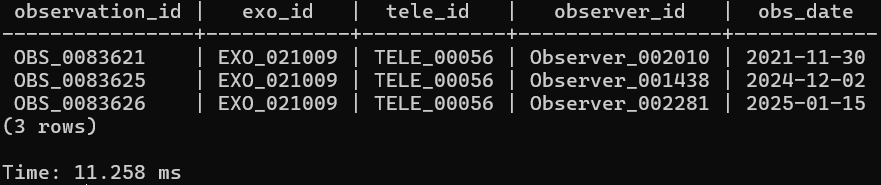
\includegraphics[width=0.85\linewidth]{images/queries/q9prep2.png}
	\caption{Результат второго запроса для подготовки к девятому запросу.}
	\label{q9prep2}
\end{figure}

Время выполнения запроса: 1.178 мс.

Были выбраны следующие поля для поиска:

\begin{itemize}
  \item A --- TELE\_00056;
  \item B --- EXO\_021009;
  \item C --- Observer\_000001 (как видно из рис. \ref{q9prep2}, у него сейчас нет этих наблюдений).
\end{itemize}

Текст запроса на SQL приведён в листинге \ref{lst:q9t}.

\begin{lstlisting}[language=SQL, caption={Текст запроса №9}, label={lst:q9t}]
UPDATE observation
SET observer_id = 'Observer_000001'
WHERE tele_id = 'TELE_00056'
  AND exo_id = 'EXO_021009';
\end{lstlisting}

Результат изображён на рис. \ref{q9r1}.

\begin{figure}[H]
	\centering
	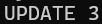
\includegraphics[width=0.85\linewidth]{images/queries/q9r1.png}
	\caption{Результат выполнения девятого запроса.}
	\label{q9r1}
\end{figure}

Реляционная формула запроса:

\[
\begin{aligned}
&\pi_{\mathrm{observation_id, exo_id, tele_id; old_observer_id, new_observer_id, obs_date}}\Big(\
&\quad \operatorname{UPDATE}*{\mathrm{observer_id} \leftarrow \mathrm{Observer_000001}}\Big(\
&\quad\quad \sigma*{\mathrm{tele_id = TELE_00056 \land exo_id = EXO_021009 \land observer_id \neq Observer_000001}}\big(\mathrm{observation}\big)\
&\quad\quad \setminus\
\pi_{\operatorname{attrs}(\mathrm{observation})}\Big(\
&\quad\quad\quad \sigma_{\mathrm{tele_id = TELE_00056 \land exo_id = EXO_021009}}\big(\mathrm{observation}\big)\
&\quad\quad\quad \ \bowtie_{\mathrm{exo_id, tele_id, obs_date}}
\sigma_{\mathrm{observer_id = Observer_000001}}\big(\mathrm{observation}\big)
\Big)\Big)\
&\Big)
\end{aligned}
\]


Последовательность выполнения запроса приведена в табл. \ref{tab:q9plan}.

\begin{table}[H]
	\centering
	\caption{Последовательность выполнения запроса 9}
	\label{tab:q9plan}
	\small
	\begin{tabularx}{\linewidth}{>{\centering\arraybackslash}p{0.9cm}>{\RaggedRight\arraybackslash}p{4.1cm}X}
		\toprule
		Шаг & Операция & Описание \\
		\midrule
		1 & Filter & Отбор наблюдений телескопа TELE\_00056 за экзопланетой EXO\_021009. \\
		2 & Anti Join & Проверка условия \texttt{NOT EXISTS}, чтобы после обновления не нарушить уникальность пары экзопланета--телескоп--наблюдатель--дата. \\
		3 & CTE & Сохранение идентификаторов обновляемых строк и старых значений observer\_id. \\
		4 & Update & Замена observer\_id на Observer\_000001 для выбранных строк. \\
		5 & Returning & Вывод идентификатора наблюдения, старого наблюдателя, нового наблюдателя и даты наблюдения. \\
		\bottomrule
	\end{tabularx}
\end{table}

Запрос сначала формирует набор строк, которые нужно изменить, и отдельно запоминает старое значение наблюдателя. Проверка \texttt{NOT EXISTS} исключает строки, для которых обновление создало бы дубликат по ограничению уникальности. Затем выполняется обновление таблицы \texttt{observation}, а блок \texttt{RETURNING} показывает результат замены.

Время выполнения запроса: 0.973 мс.

На рис. \ref{q9change} видно сравнение старых и новых значений поля observer.

\begin{figure}[H]
	\centering
	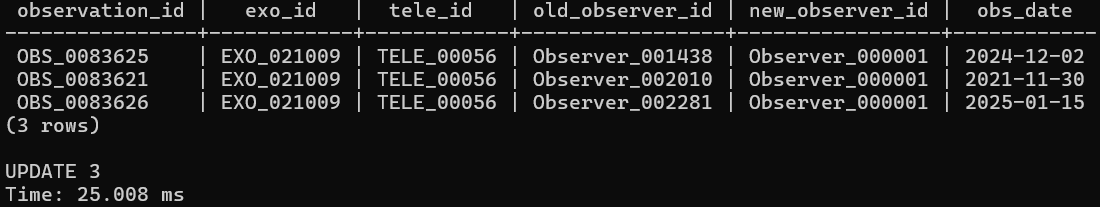
\includegraphics[width=0.85\linewidth]{images/queries/q9change.png}
	\caption{Результат выполнения второго запроса (сравнение значений до и после).}
	\label{q9change}
\end{figure}

Далее был введён ещё один запрос, чтобы проверить, что значения действительно обновились:

\begin{lstlisting}[language=SQL, caption={Проверочный запрос после выполнения запроса №9}, label={lst:q9check}]
SELECT
    observation_id,
    exo_id,
    tele_id,
    observer_id,
    obs_date
FROM observation
WHERE tele_id = 'TELE_00056'
  AND exo_id = 'EXO_021009'
ORDER BY obs_date, observation_id;
\end{lstlisting}

Как видно на рис. \ref{q9r}, значения в таблице действительно обновились.

\begin{figure}[H]
	\centering
	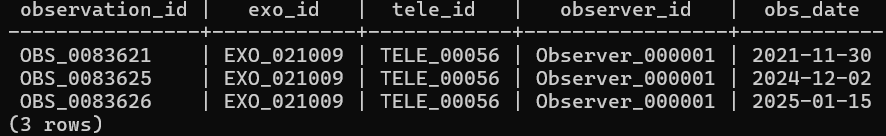
\includegraphics[width=0.85\linewidth]{images/queries/q9r.png}
	\caption{Проверка изменённых значений в таблице после девятого запроса.}
	\label{q9r}
\end{figure}

Время выполнения запроса: 1.093 мс.

\newpage

\section*{Заключение}
\addcontentsline{toc}{section}{Заключение}

В ходе работы был выполнен анализ предметной области <<Каталогизация экзопланет>>, определены цели функционирования базы данных, выявлены основные сущности, их атрибуты и связи. На основе анализа построена ER-диаграмма в нотации Чена, спроектирована схема базы данных и описаны таблицы с обоснованием выбранных типов атрибутов.

Схема базы данных реализована в СУБД PostgreSQL. Для заполнения базы данных написана программа на языке Python с использованием библиотеки \textit{psycopg2}. В итоговой базе содержится 273~166 записей в 9 таблицах, описывающих галактики, звёздные скопления, звёздные и планетарные системы, звёзды, экзопланеты, телескопы, наблюдателей и наблюдения.

Выполнены 9 запросов к базе данных. Для каждого запроса приведены SQL-текст, реляционная формула, последовательность выполнения, текстовое пояснение работы запроса, время выполнения и фрагмент результата. Для запросов, требующих визуального представления данных, построены графики результатов средствами языка R.

Разработанная база данных может служить основой для хранения и анализа сведений об экзопланетах, связанных с ними астрономических объектах и событиях наблюдения. Полученная структура позволяет выполнять выборки по характеристикам экзопланет, телескопов, звёзд, галактик и наблюдателей, а также использовать накопленные данные для аналитических отчётов.

Работа выполнялась на ноутбуке HP Pavilion Gaming Laptop 16-a0xxx с процессором Intel(R) Core(TM) i7-10750H CPU, 6 ядер, 2.60 ГГц, и 16 ГБ оперативной памяти. Запросы выполнялись в СУБД PostgreSQL; генерация данных реализована на языке Python, визуализация результатов выполнена средствами языка R. Среда разработки --- Visual Studio Code.

\newpage

\begin{thebibliography}{9}
		\bibitem{exoplanet} NASA. Exoplanets - NASA Science [Электронный ресурс] / Chelsea Gohd, Diana Logreira --- URL: \url{https://science.nasa.gov/exoplanets/} (дата обращения: 05.02.2026).
		
		\bibitem{planet} NASA. What is a Planet? [Электронный ресурс] / Stephen Carney, Diana Logreira --- URL: \url{https://science.nasa.gov/solar-system/planets/what-is-a-planet/} (дата обращения: 05.02.2026).
		
		\bibitem{lasilla} ESA. La Silla Observatory [Электронный ресурс] / URL: \url{https://www.eso.org/public/teles-instr/lasilla/} (дата обращения: 10.02.2026).
		
		\bibitem{nasa-exoplanet-catalog} NASA. Exoplanet Catalog [Электронный ресурс] / URL: \url{https://science.nasa.gov/exoplanets/exoplanet-catalog/} (дата обращения: 10.02.2026).
		
		\bibitem{oec} \url{https://www.openexoplanetcatalogue.com/} (дата обращения: 10.02.2026).
		
		\bibitem{catalog-eu} \url{https://exoplanet.eu/catalog/} (дата обращения: 10.02.2026).
		
		\bibitem{kepler} \url{https://science.nasa.gov/resource/kepler-186f-the-first-earth-size-planet-in-the-habitable-zone-artists-concept/} (дата обращения: 10.02.2026).
		
		\bibitem{methods} \url{https://science.nasa.gov/exoplanets/how-we-find-and-characterize/} (дата обращения: 10.02.2026).
		
		\bibitem{exoDiscovery} NASA. In Depth: Exoplanets [Электронный ресурс] / Stephen Carney, Diana Logreira --- URL: \url{https://science.nasa.gov/exoplanets/facts/} (дата обращения: 05.02.2026).
		
		\bibitem{exoTypes} NASA. What is an Exoplanet? [Электронный ресурс] / Stephen Carney, Diana Logreira --- URL: \url{https://science.nasa.gov/exoplanets/planet-types/} (дата обращения: 05.02.2026).
		
		\bibitem{webb} \url{https://science.nasa.gov/mission/webb/}
		
		\bibitem{largeScale} NASA. Large Scale Structures - NASA Science [Электронный ресурс] / Jeanette Kazmierczak, Diana Logreira --- URL: \url{https://science.nasa.gov/universe/galaxies/large-scale-structures/} (дата обращения: 07.02.2026).
		
		\bibitem{entites} Понятие предметной области. Определение сущностей, связей и их свойств. [Электронный ресурс] / URL: \url{https://studfile.net/preview/9568409/page:26/} (дата образщения: 07.02.2026).
		
		\bibitem{citizen-science-ru} \url{https://citizen-science.ru/about/} (дата обращения: 07.02.2026).
		
		\bibitem{cows} Raghu Ramakrishnan, Johannes Gehrke. Database Management Systems / McGraw-Hill Higher Education --- 2 издание --- Нью-Йорк, 2002 --- 931 c. --- 26--27, 136--138 c. --- 9780071121132 (дата обращения: 11.02.2026).
		
		\bibitem{manga} Takahashi, Mana, Azuma, Shoko. The Manga Guide to Databases. / TrendPro CO. LTD --- Токио, 2009 --- 228 с. --- 118 с. --- 1593271905 (дата обращения: 08.02.2026).
		
		\bibitem{M4} NASA. Artist’s View of Planetary System in Globular Cluster M4 / URL: \url{https://science.nasa.gov/asset/hubble/artists-view-of-planetary-system-in-globular-cluster-m4/} (дата обращения: 11.02.2026).
		
		\bibitem{rel-bd-book} В.Ю. Кара-Ушанов. Реляционная модель данных / В.Ю. Кара-Ушанов, А.В. Овчинникова --- Информационный портал УрФУ --- Екатеринбург, 2017 --- 6--7 с. (дата обращения: 11.02.2026).
		
		\bibitem{stellar-classes} \url{https://www.britannica.com/science/stellar-classification}
		
		\bibitem{first-exoplanet-date} \url{https://science.nasa.gov/universe/exoplanets/discovery-alert-with-six-new-worlds-5500-discovery-milestone-passed/#:~:text=The%20Discovery,-With%20the%20discovery&text=Just%20about%2031%20years%20ago,celebrated%20passing%205%2C000%20exoplanets%20discovered.}
		
		\bibitem{names-standards} \url{https://www.scientificamerican.com/article/how-do-we-name-the-stars/#:~:text=These%20more%20modern%20datasets%20(and,Betelgeuse.}
	\end{thebibliography}

\newpage

\section*{Приложение А. Исходный тест программы генерации базы данных}
\addcontentsline{toc}{section}{Приложение А. Исходный тест программы генерации базы данных}

\begin{lstlisting}
-- schema.sql

-- ========================
-- ENUM TYPES
-- ========================

CREATE TYPE tele_type_enum AS ENUM ('space', 'ground');

CREATE TYPE exo_type_enum AS ENUM (
    'gas_giant',
    'neptunian',
    'superearth',
    'terrestrial'
);

CREATE TYPE star_class_enum AS ENUM (
    'O','B','A','F','G','K','M','W','L','D'
);

CREATE TYPE country_enum AS ENUM (
'Afghanistan','Albania','Algeria','Andorra','Angola','Antigua and Barbuda',
'Argentina','Armenia','Australia','Austria','Azerbaijan',
'Bahamas','Bahrain','Bangladesh','Barbados','Belarus','Belgium','Belize',
'Benin','Bhutan','Bolivia','Bosnia and Herzegovina','Botswana','Brazil',
'Brunei','Bulgaria','Burkina Faso','Burundi',
'Cabo Verde','Cambodia','Cameroon','Canada','Central African Republic',
'Chad','Chile','China','Colombia','Comoros','Congo (Congo-Brazzaville)',
'Costa Rica','Croatia','Cuba','Cyprus','Czechia',
'Democratic Republic of the Congo','Denmark','Djibouti','Dominica',
'Dominican Republic',
'Ecuador','Egypt','El Salvador','Equatorial Guinea','Eritrea','Estonia',
'Eswatini','Ethiopia',
'Fiji','Finland','France',
'Gabon','Gambia','Georgia','Germany','Ghana','Greece','Grenada',
'Guatemala','Guinea','Guinea-Bissau','Guyana',
'Haiti','Honduras','Hungary',
'Iceland','India','Indonesia','Iran','Iraq','Ireland','Israel','Italy',
'Jamaica','Japan','Jordan',
'Kazakhstan','Kenya','Kiribati','Kuwait','Kyrgyzstan',
'Laos','Latvia','Lebanon','Lesotho','Liberia','Libya','Liechtenstein',
'Lithuania','Luxembourg',
'Madagascar','Malawi','Malaysia','Maldives','Mali','Malta',
'Marshall Islands','Mauritania','Mauritius','Mexico','Micronesia',
'Moldova','Monaco','Mongolia','Montenegro','Morocco','Mozambique',
'Myanmar',
'Namibia','Nauru','Nepal','Netherlands','New Zealand','Nicaragua','Niger',
'Nigeria','North Korea','North Macedonia','Norway',
'Oman',
'Pakistan','Palau','Panama','Papua New Guinea','Paraguay','Peru',
'Philippines','Poland','Portugal',
'Qatar',
'Romania','Russia','Rwanda',
'Saint Kitts and Nevis','Saint Lucia',
'Saint Vincent and the Grenadines','Samoa','San Marino',
'Sao Tome and Principe','Saudi Arabia','Senegal','Serbia','Seychelles',
'Sierra Leone','Singapore','Slovakia','Slovenia','Solomon Islands',
'Somalia','South Africa','South Korea','South Sudan','Spain','Sri Lanka',
'Sudan','Suriname','Sweden','Switzerland','Syria',
'Taiwan','Tajikistan','Tanzania','Thailand','Timor-Leste','Togo','Tonga',
'Trinidad and Tobago','Tunisia','Turkey','Turkmenistan','Tuvalu',
'Uganda','Ukraine','United Arab Emirates','United Kingdom',
'United States','Uruguay','Uzbekistan',
'Vanuatu','Vatican City','Venezuela','Vietnam',
'Yemen',
'Zambia','Zimbabwe'
);

-- ========================
-- CORE TABLES
-- ========================

CREATE TABLE galaxy (
    galaxy_id VARCHAR(30) PRIMARY KEY,
    conf_plan INT NOT NULL CHECK (conf_plan >= 0),
    hab_plan  INT NOT NULL CHECK (hab_plan >= 0 AND hab_plan <= conf_plan),
    dist      DECIMAL(12, 6) NOT NULL CHECK (dist >= 0)
);

CREATE TABLE cluster (
    cluster_id  VARCHAR(30) PRIMARY KEY,
    stars_count INT NOT NULL CHECK (stars_count >= 10),
    conf_plan   INT NOT NULL CHECK (conf_plan >= 0),
    hab_plan    INT NOT NULL CHECK (hab_plan >= 0 AND hab_plan <= conf_plan),
    dist        DECIMAL(12, 6) NOT NULL CHECK (dist >= 0),
    galaxy_id   VARCHAR(30) NOT NULL
        REFERENCES galaxy(galaxy_id) ON DELETE CASCADE
);

CREATE TABLE stellar_system (
    stellar_id  VARCHAR(30) PRIMARY KEY,
    stars_count INT NOT NULL CHECK (stars_count >= 1),
    conf_plan   INT NOT NULL CHECK (conf_plan >= 0),
    hab_plan    INT NOT NULL CHECK (hab_plan >= 0 AND hab_plan <= conf_plan),
    dist        DECIMAL(12, 6) NOT NULL CHECK (dist >= 0),
    cluster_id  VARCHAR(30) NOT NULL
        REFERENCES cluster(cluster_id) ON DELETE CASCADE
);

CREATE TABLE plan_system (
    system_id    VARCHAR(30) PRIMARY KEY,
    conf_plan    INT NOT NULL CHECK (conf_plan >= 1),
    hab_plan     INT NOT NULL CHECK (hab_plan >= 0 AND hab_plan <= conf_plan),
    distance     DECIMAL(12, 6) NOT NULL CHECK (distance >= 0),
    stell_sys_id VARCHAR(30) NOT NULL
        REFERENCES stellar_system(stellar_id) ON DELETE CASCADE
);

-- ========================
-- OBJECTS
-- ========================

CREATE TABLE star (
    star_id  VARCHAR(30) PRIMARY KEY,
    class    star_class_enum NOT NULL,
    mass     DECIMAL(5, 2) NOT NULL CHECK (mass > 0),
    radius   DECIMAL(10, 4) NOT NULL CHECK (radius > 0),
    temp     INT NOT NULL CHECK (temp > 0),
    dist     DECIMAL(16, 6) NOT NULL CHECK (dist >= 0),
    sys_id   VARCHAR(30) NOT NULL
        REFERENCES plan_system(system_id) ON DELETE CASCADE
);

CREATE TABLE exoplanet (
    exo_id        VARCHAR(30) PRIMARY KEY,
    mass          DECIMAL(10, 4) NOT NULL CHECK (mass > 0),
    radius        DECIMAL(10, 4) NOT NULL CHECK (radius > 0),
    orb_period    DECIMAL(10, 4) NOT NULL CHECK (orb_period > 0),
    exo_type      exo_type_enum NOT NULL,
    dist          DECIMAL(12, 6) NOT NULL CHECK (dist >= 0),
    discov_date   DATE NOT NULL CHECK (
        discov_date BETWEEN DATE '1992-01-01' AND CURRENT_DATE
    ),
    last_obs_date DATE NOT NULL CHECK (
        last_obs_date BETWEEN discov_date AND CURRENT_DATE
    ),
    sys_id        VARCHAR(30) NOT NULL
        REFERENCES plan_system(system_id) ON DELETE CASCADE
);

CREATE TABLE telescope (
    tele_id VARCHAR(47) PRIMARY KEY,
    tele_type tele_type_enum NOT NULL,
    aper DECIMAL(6,2) NOT NULL CHECK (aper > 0),
    com_year INT NOT NULL CHECK (
        com_year BETWEEN 1609 AND EXTRACT(YEAR FROM CURRENT_DATE)::INT
    ),
    oper VARCHAR(81) NOT NULL,
    discov_plan INT NOT NULL CHECK (discov_plan >= 0)
);

CREATE TABLE observer (
    observer_id VARCHAR(100) PRIMARY KEY,
    bday        DATE NOT NULL CHECK (
        bday BETWEEN DATE '1609-01-01' AND CURRENT_DATE
    ),
    country     country_enum NOT NULL,
    discovs     INT NOT NULL CHECK (discovs >= 0)
);

CREATE TABLE observation (
    observation_id VARCHAR(30) PRIMARY KEY,
    exo_id         VARCHAR(30) NOT NULL
        REFERENCES exoplanet(exo_id) ON DELETE CASCADE,
    tele_id        VARCHAR(47) NOT NULL
        REFERENCES telescope(tele_id) ON DELETE CASCADE,
    observer_id    VARCHAR(100) NOT NULL
        REFERENCES observer(observer_id) ON DELETE CASCADE,
    obs_date       DATE NOT NULL CHECK (
        obs_date BETWEEN DATE '1992-01-01' AND CURRENT_DATE
    ),
    CONSTRAINT observation_unique_event
        UNIQUE (exo_id, tele_id, observer_id, obs_date)
);
\end{lstlisting}

\newpage

\section*{Приложение Б. Исходный текст программы генерации тестовых данных}
\addcontentsline{toc}{section}{Приложение Б. Исходный текст программы генерации тестовых данных}
\label{b}

\begin{lstlisting}
import psycopg2
from datetime import date, timedelta
import random

conn = psycopg2.connect(dbname="mydb", user="postgres")
cur = conn.cursor()

print("Очистка таблиц...")

cur.execute("""
    TRUNCATE TABLE
        observation,
        exoplanet,
        star,
        telescope,
        observer,
        plan_system,
        stellar_system,
        cluster,
        galaxy
    CASCADE;
""")

TODAY = date.today()


def random_date(start_date, end_date):
    days = (end_date - start_date).days
    return start_date + timedelta(days=random.randint(0, days))


def random_decimal(min_value, max_value):
    return random.uniform(min_value, max_value)


def make_id(prefix, number, width=5):
    return f"{prefix}_{number:0{width}d}"


\# Случайное количество записей
\# с контролем общей суммы 200k–300k
\# ===========================
TARGET_MIN = 200_000
TARGET_MAX = 300_000

while True:
    GALAXIES_COUNT = random.randint(30, 70)
    CLUSTERS_COUNT = random.randint(300, 700)
    STELLAR_SYSTEMS_COUNT = random.randint(3000, 7000)
    PLAN_SYSTEMS_COUNT = random.randint(15000, 30000)
    STARS_COUNT = random.randint(25000, 50000)
    EXOPLANETS_COUNT = random.randint(30000, 50000)
    TELESCOPES_COUNT = random.randint(200, 500)
    OBSERVERS_COUNT = random.randint(7000, 15000)

    estimated_observations = EXOPLANETS_COUNT * 4

    estimated_total = (
        GALAXIES_COUNT
        + CLUSTERS_COUNT
        + STELLAR_SYSTEMS_COUNT
        + PLAN_SYSTEMS_COUNT
        + STARS_COUNT
        + EXOPLANETS_COUNT
        + TELESCOPES_COUNT
        + OBSERVERS_COUNT
        + estimated_observations
    )

    if TARGET_MIN <= estimated_total <= TARGET_MAX:
        break

\# Гарантия, что хватит звёзд: минимум 10 звёзд на каждое скопление
if STARS_COUNT < CLUSTERS_COUNT * 10:
    STARS_COUNT = CLUSTERS_COUNT * 10

\# Гарантия, что хватит планетарных систем: минимум 1 на каждое скопление
if PLAN_SYSTEMS_COUNT < CLUSTERS_COUNT:
    PLAN_SYSTEMS_COUNT = CLUSTERS_COUNT

\# Гарантия, что хватит звёздных систем: минимум 1 на каждое скопление
if STELLAR_SYSTEMS_COUNT < CLUSTERS_COUNT:
    STELLAR_SYSTEMS_COUNT = CLUSTERS_COUNT

print("Случайно выбранное количество записей:")
print(f"Галактик: {GALAXIES_COUNT}")
print(f"Скоплений: {CLUSTERS_COUNT}")
print(f"Звёздных систем: {STELLAR_SYSTEMS_COUNT}")
print(f"Планетных систем: {PLAN_SYSTEMS_COUNT}")
print(f"Звёзд: {STARS_COUNT}")
print(f"Экзопланет: {EXOPLANETS_COUNT}")
print(f"Телескопов: {TELESCOPES_COUNT}")
print(f"Наблюдателей: {OBSERVERS_COUNT}")
print(f"Примерная сумма: {estimated_total}")

\# ===========================
\# ENUM значения
\# ===========================
exo_types = [
    'gas_giant',
    'neptunian',
    'superearth',
    'terrestrial'
]

star_classes = [
    'O', 'B', 'A', 'F', 'G', 'K', 'M', 'W', 'L', 'D'
]

tele_types = [
    'space',
    'ground'
]

countries = [
'Afghanistan','Albania','Algeria','Andorra','Angola','Antigua and Barbuda',
'Argentina','Armenia','Australia','Austria','Azerbaijan',
'Bahamas','Bahrain','Bangladesh','Barbados','Belarus','Belgium','Belize',
'Benin','Bhutan','Bolivia','Bosnia and Herzegovina','Botswana','Brazil',
'Brunei','Bulgaria','Burkina Faso','Burundi',
'Cabo Verde','Cambodia','Cameroon','Canada','Central African Republic',
'Chad','Chile','China','Colombia','Comoros','Congo (Congo-Brazzaville)',
'Costa Rica','Croatia','Cuba','Cyprus','Czechia',
'Democratic Republic of the Congo','Denmark','Djibouti','Dominica',
'Dominican Republic',
'Ecuador','Egypt','El Salvador','Equatorial Guinea','Eritrea','Estonia',
'Eswatini','Ethiopia',
'Fiji','Finland','France',
'Gabon','Gambia','Georgia','Germany','Ghana','Greece','Grenada',
'Guatemala','Guinea','Guinea-Bissau','Guyana',
'Haiti','Honduras','Hungary',
'Iceland','India','Indonesia','Iran','Iraq','Ireland','Israel','Italy',
'Jamaica','Japan','Jordan',
'Kazakhstan','Kenya','Kiribati','Kuwait','Kyrgyzstan',
'Laos','Latvia','Lebanon','Lesotho','Liberia','Libya','Liechtenstein',
'Lithuania','Luxembourg',
'Madagascar','Malawi','Malaysia','Maldives','Mali','Malta',
'Marshall Islands','Mauritania','Mauritius','Mexico','Micronesia',
'Moldova','Monaco','Mongolia','Montenegro','Morocco','Mozambique',
'Myanmar',
'Namibia','Nauru','Nepal','Netherlands','New Zealand','Nicaragua','Niger',
'Nigeria','North Korea','North Macedonia','Norway',
'Oman',
'Pakistan','Palau','Panama','Papua New Guinea','Paraguay','Peru',
'Philippines','Poland','Portugal',
'Qatar',
'Romania','Russia','Rwanda',
'Saint Kitts and Nevis','Saint Lucia',
'Saint Vincent and the Grenadines','Samoa','San Marino',
'Sao Tome and Principe','Saudi Arabia','Senegal','Serbia','Seychelles',
'Sierra Leone','Singapore','Slovakia','Slovenia','Solomon Islands',
'Somalia','South Africa','South Korea','South Sudan','Spain','Sri Lanka',
'Sudan','Suriname','Sweden','Switzerland','Syria',
'Taiwan','Tajikistan','Tanzania','Thailand','Timor-Leste','Togo','Tonga',
'Trinidad and Tobago','Tunisia','Turkey','Turkmenistan','Tuvalu',
'Uganda','Ukraine','United Arab Emirates','United Kingdom',
'United States','Uruguay','Uzbekistan',
'Vanuatu','Vatican City','Venezuela','Vietnam',
'Yemen',
'Zambia','Zimbabwe'
]

operators = [
    'NASA',
    'ESA',
    'Roscosmos',
    'JAXA',
    'CNSA',
    'ESO',
    'ISRO',
    'DLR',
    'CNES',
    'Private Observatory Network',
    'International Space Research Group',
    'Global Telescope Association'
]

\# ===========================
\# 1. Галактики
\# ===========================
print("Галактики...")

galaxy_ids = []

for i in range(1, GALAXIES_COUNT + 1):
    galaxy_id = make_id("GAL", i, 4)

    conf_plan = random.randint(10, 5000)
    hab_plan = random.randint(0, conf_plan)

    cur.execute("""
        INSERT INTO galaxy
        (galaxy_id, conf_plan, hab_plan, dist)
        VALUES (%s, %s, %s, %s);
    """, (
        galaxy_id,
        conf_plan,
        hab_plan,
        random_decimal(0, 1000000)
    ))

    galaxy_ids.append(galaxy_id)

\# ===========================
\# 2. Скопления
\# ===========================
print("Скопления...")

cluster_ids = []

for i in range(1, CLUSTERS_COUNT + 1):
    cluster_id = make_id("CLS", i, 5)

    conf_plan = random.randint(5, 2000)
    hab_plan = random.randint(0, conf_plan)

    cur.execute("""
        INSERT INTO cluster
        (cluster_id, stars_count, conf_plan, hab_plan, dist, galaxy_id)
        VALUES (%s, %s, %s, %s, %s, %s);
    """, (
        cluster_id,
        random.randint(10, 100000),
        conf_plan,
        hab_plan,
        random_decimal(0, 500000),
        random.choice(galaxy_ids)
    ))

    cluster_ids.append(cluster_id)

\# ===========================
\# 3. Звёздные системы
\# ===========================
print("Звёздные системы...")

stellar_ids = []
stellar_to_cluster = {}
cluster_stellar_ids = {cluster_id: [] for cluster_id in cluster_ids}

stellar_counter = 1

\# Минимум 1 звёздная система на каждое скопление
for cluster_id in cluster_ids:
    stellar_id = make_id("STELLAR", stellar_counter, 5)
    stellar_counter += 1

    conf_plan = random.randint(1, 300)
    hab_plan = random.randint(0, conf_plan)

    cur.execute("""
        INSERT INTO stellar_system
        (stellar_id, stars_count, conf_plan, hab_plan, dist, cluster_id)
        VALUES (%s, %s, %s, %s, %s, %s);
    """, (
        stellar_id,
        random.randint(1, 8),
        conf_plan,
        hab_plan,
        random_decimal(0, 100000),
        cluster_id
    ))

    stellar_ids.append(stellar_id)
    stellar_to_cluster[stellar_id] = cluster_id
    cluster_stellar_ids[cluster_id].append(stellar_id)

\# Остальные звёздные системы случайно
while stellar_counter <= STELLAR_SYSTEMS_COUNT:
    stellar_id = make_id("STELLAR", stellar_counter, 5)
    stellar_counter += 1

    cluster_id = random.choice(cluster_ids)

    conf_plan = random.randint(1, 300)
    hab_plan = random.randint(0, conf_plan)

    cur.execute("""
        INSERT INTO stellar_system
        (stellar_id, stars_count, conf_plan, hab_plan, dist, cluster_id)
        VALUES (%s, %s, %s, %s, %s, %s);
    """, (
        stellar_id,
        random.randint(1, 8),
        conf_plan,
        hab_plan,
        random_decimal(0, 100000),
        cluster_id
    ))

    stellar_ids.append(stellar_id)
    stellar_to_cluster[stellar_id] = cluster_id
    cluster_stellar_ids[cluster_id].append(stellar_id)

\# ===========================
\# 4. Планетные системы
\# ===========================
print("Планетные системы...")

plan_system_ids = []
plan_system_to_cluster = {}
cluster_plan_system_ids = {cluster_id: [] for cluster_id in cluster_ids}

system_counter = 1

\# Минимум 1 планетарная система на каждое звёздное скопление
for cluster_id in cluster_ids:
    system_id = make_id("SYS", system_counter, 6)
    system_counter += 1

    stellar_id = random.choice(cluster_stellar_ids[cluster_id])

    conf_plan = random.randint(1, 20)
    hab_plan = random.randint(0, conf_plan)

    cur.execute("""
        INSERT INTO plan_system
        (system_id, conf_plan, hab_plan, distance, stell_sys_id)
        VALUES (%s, %s, %s, %s, %s);
    """, (
        system_id,
        conf_plan,
        hab_plan,
        random_decimal(0, 100000),
        stellar_id
    ))

    plan_system_ids.append(system_id)
    plan_system_to_cluster[system_id] = cluster_id
    cluster_plan_system_ids[cluster_id].append(system_id)

\# Остальные планетарные системы случайно
while system_counter <= PLAN_SYSTEMS_COUNT:
    system_id = make_id("SYS", system_counter, 6)
    system_counter += 1

    stellar_id = random.choice(stellar_ids)
    cluster_id = stellar_to_cluster[stellar_id]

    conf_plan = random.randint(1, 20)
    hab_plan = random.randint(0, conf_plan)

    cur.execute("""
        INSERT INTO plan_system
        (system_id, conf_plan, hab_plan, distance, stell_sys_id)
        VALUES (%s, %s, %s, %s, %s);
    """, (
        system_id,
        conf_plan,
        hab_plan,
        random_decimal(0, 100000),
        stellar_id
    ))

    plan_system_ids.append(system_id)
    plan_system_to_cluster[system_id] = cluster_id
    cluster_plan_system_ids[cluster_id].append(system_id)

\# ===========================
\# 5. Звёзды
\# ===========================
print("Звёзды...")


def generate_star_params():
    star_class = random.choice(star_classes)

    if star_class == 'O':
        mass = random_decimal(16, 90)
        radius = random_decimal(6, 20)
        temp = random.randint(30000, 50000)

    elif star_class == 'B':
        mass = random_decimal(2.1, 16)
        radius = random_decimal(1.8, 6)
        temp = random.randint(10000, 30000)

    elif star_class == 'A':
        mass = random_decimal(1.4, 2.1)
        radius = random_decimal(1.4, 2.5)
        temp = random.randint(7500, 10000)

    elif star_class == 'F':
        mass = random_decimal(1.04, 1.4)
        radius = random_decimal(1.15, 1.4)
        temp = random.randint(6000, 7500)

    elif star_class == 'G':
        mass = random_decimal(0.8, 1.04)
        radius = random_decimal(0.9, 1.15)
        temp = random.randint(5200, 6000)

    elif star_class == 'K':
        mass = random_decimal(0.45, 0.8)
        radius = random_decimal(0.7, 0.9)
        temp = random.randint(3700, 5200)

    elif star_class == 'M':
        mass = random_decimal(0.08, 0.45)
        radius = random_decimal(0.1, 0.7)
        temp = random.randint(2400, 3700)

    else:
        mass = random_decimal(0.1, 10)
        radius = random_decimal(0.01, 5)
        temp = random.randint(1000, 100000)

    return star_class, mass, radius, temp


def insert_star(star_id, system_id):
    star_class, mass, radius, temp = generate_star_params()

    cur.execute("""
        INSERT INTO star
        (star_id, class, mass, radius, temp, dist, sys_id)
        VALUES (%s, %s, %s, %s, %s, %s, %s);
    """, (
        star_id,
        star_class,
        mass,
        radius,
        temp,
        random_decimal(0, 100000),
        system_id
    ))


star_ids = []
star_counter = 1

\# Минимум 10 звёзд в каждом звёздном скоплении
for cluster_id in cluster_ids:
    for _ in range(10):
        star_id = make_id("STAR", star_counter, 6)
        star_counter += 1

        system_id = random.choice(cluster_plan_system_ids[cluster_id])

        insert_star(star_id, system_id)
        star_ids.append(star_id)

\# Остальные звёзды случайно
while star_counter <= STARS_COUNT:
    star_id = make_id("STAR", star_counter, 6)
    star_counter += 1

    system_id = random.choice(plan_system_ids)

    insert_star(star_id, system_id)
    star_ids.append(star_id)

\# ===========================
\# 6. Экзопланеты
\# ===========================
print("Экзопланеты...")

exo_ids = []
exo_discovery_dates = {}

for i in range(1, EXOPLANETS_COUNT + 1):
    exo_id = make_id("EXO", i, 6)
    exo_type = random.choice(exo_types)

    if exo_type == 'gas_giant':
        mass = random_decimal(50, 5000)
        radius = random_decimal(5, 20)

    elif exo_type == 'neptunian':
        mass = random_decimal(10, 50)
        radius = random_decimal(2, 6)

    elif exo_type == 'superearth':
        mass = random_decimal(2, 10)
        radius = random_decimal(1.2, 2.5)

    else:
        mass = random_decimal(0.1, 2)
        radius = random_decimal(0.3, 1.5)

    discov_date = random_date(date(1992, 1, 1), TODAY)
    last_obs_date = random_date(discov_date, TODAY)

    cur.execute("""
        INSERT INTO exoplanet
        (exo_id, mass, radius, orb_period, exo_type, dist,
         discov_date, last_obs_date, sys_id)
        VALUES (%s, %s, %s, %s, %s, %s, %s, %s, %s);
    """, (
        exo_id,
        mass,
        radius,
        random_decimal(0.5, 5000),
        exo_type,
        random_decimal(0, 100000),
        discov_date,
        last_obs_date,
        random.choice(plan_system_ids)
    ))

    exo_ids.append(exo_id)
    exo_discovery_dates[exo_id] = discov_date

\# ===========================
\# 7. Телескопы
\# ===========================
print("Телескопы...")

tele_ids = []

for i in range(1, TELESCOPES_COUNT + 1):
    tele_id = make_id("TELE", i, 5)

    tele_type = random.choice(tele_types)

    if tele_type == 'space':
        aper = random_decimal(0.2, 10)
        com_year = random.randint(1960, TODAY.year)
    else:
        aper = random_decimal(0.5, 40)
        com_year = random.randint(1609, TODAY.year)

    cur.execute("""
        INSERT INTO telescope
        (tele_id, tele_type, aper, com_year, oper, discov_plan)
        VALUES (%s, %s, %s, %s, %s, %s);
    """, (
        tele_id,
        tele_type,
        aper,
        com_year,
        random.choice(operators),
        0
    ))

    tele_ids.append(tele_id)

\# ===========================
\# 8. Наблюдатели
\# ===========================
print("Наблюдатели...")

observer_ids = []

for i in range(1, OBSERVERS_COUNT + 1):
    observer_id = f"Observer_{i:06d}"

    cur.execute("""
        INSERT INTO observer
        (observer_id, bday, country, discovs)
        VALUES (%s, %s, %s, %s);
    """, (
        observer_id,
        random_date(date(1930, 1, 1), date(2005, 12, 31)),
        random.choice(countries),
        0
    ))

    observer_ids.append(observer_id)

\# ===========================
\# 9. Наблюдения
\# ===========================
print("Наблюдения...")

observation_ids = []
used_observations = set()

telescope_discovs = {tele_id: 0 for tele_id in tele_ids}
observer_discovs = {observer_id: 0 for observer_id in observer_ids}

obs_counter = 1

for exo_id in exo_ids:
    observations_for_planet = random.randint(1, 7)

    for _ in range(observations_for_planet):
        tele_id = random.choice(tele_ids)
        observer_id = random.choice(observer_ids)

        obs_date = random_date(exo_discovery_dates[exo_id], TODAY)

        unique_key = (exo_id, tele_id, observer_id, obs_date)

        attempts = 0
        while unique_key in used_observations and attempts < 20:
            tele_id = random.choice(tele_ids)
            observer_id = random.choice(observer_ids)
            obs_date = random_date(exo_discovery_dates[exo_id], TODAY)

            unique_key = (exo_id, tele_id, observer_id, obs_date)
            attempts += 1

        if unique_key in used_observations:
            continue

        used_observations.add(unique_key)

        observation_id = make_id("OBS", obs_counter, 7)
        obs_counter += 1

        cur.execute("""
            INSERT INTO observation
            (observation_id, exo_id, tele_id, observer_id, obs_date)
            VALUES (%s, %s, %s, %s, %s);
        """, (
            observation_id,
            exo_id,
            tele_id,
            observer_id,
            obs_date
        ))

        observation_ids.append(observation_id)

        telescope_discovs[tele_id] += 1
        observer_discovs[observer_id] += 1

\# ===========================
\# 10. Обновление статистики
\# ===========================
print("Обновление статистики...")

for tele_id, count in telescope_discovs.items():
    cur.execute("""
        UPDATE telescope
        SET discov_plan = %s
        WHERE tele_id = %s;
    """, (
        count,
        tele_id
    ))

for observer_id, count in observer_discovs.items():
    cur.execute("""
        UPDATE observer
        SET discovs = %s
        WHERE observer_id = %s;
    """, (
        count,
        observer_id
    ))

\# ===========================
\# Завершение
\# ===========================
conn.commit()
cur.close()
conn.close()

total_records = (
    len(galaxy_ids)
    + len(cluster_ids)
    + len(stellar_ids)
    + len(plan_system_ids)
    + len(star_ids)
    + len(exo_ids)
    + len(tele_ids)
    + len(observer_ids)
    + len(observation_ids)
)

print("Готово!")
print(f"Галактик: {len(galaxy_ids)}")
print(f"Скоплений: {len(cluster_ids)}")
print(f"Звёздных систем: {len(stellar_ids)}")
print(f"Планетных систем: {len(plan_system_ids)}")
print(f"Звёзд: {len(star_ids)}")
print(f"Экзопланет: {len(exo_ids)}")
print(f"Телескопов: {len(tele_ids)}")
print(f"Наблюдателей: {len(observer_ids)}")
print(f"Наблюдений: {len(observation_ids)}")
print(f"Всего записей: {total_records}")

\# print()
\# print("Проверочные SQL-запросы:")
\# print("""
\# 1. Проверка, что в каждом скоплении есть минимум 1 планетарная система:

\# SELECT 
\#     c.cluster_id,
\#     COUNT(DISTINCT ps.system_id) AS planet_systems_count
\# FROM cluster c
\# LEFT JOIN stellar_system ss 
\#     ON ss.cluster_id = c.cluster_id
\# LEFT JOIN plan_system ps 
\#     ON ps.stell_sys_id = ss.stellar_id
\# GROUP BY c.cluster_id
\# HAVING COUNT(DISTINCT ps.system_id) < 1;

\# 2. Проверка, что в каждом скоплении есть минимум 10 звёзд:

\# SELECT 
\#     c.cluster_id,
\#     COUNT(s.star_id) AS stars_count
\# FROM cluster c
\# LEFT JOIN stellar_system ss 
\#     ON ss.cluster_id = c.cluster_id
\# LEFT JOIN plan_system ps 
\#     ON ps.stell_sys_id = ss.stellar_id
\# LEFT JOIN star s 
\#     ON s.sys_id = ps.system_id
\# GROUP BY c.cluster_id
\# HAVING COUNT(s.star_id) < 10;
\# """)
\end{lstlisting}

\end{document}
